\chapter{Soluzione proposta}
\label{SoluzioneProposta}
\thispagestyle{empty}

%\vspace{0.5cm}

\noindent In questo capitolo descriviamo la soluzione che abbiamo proposto per risolvere il problema del tampering detection, formulato nel Capitolo \ref{FormulazioneProblema}.\\
Nel Paragrafo \ref{indicatori} descriviamo quali sono gli indicatori che abbiamo deciso di monitorare per individuare gli eventi di tampering.\\
Nel Paragrafo  \ref{monitoraggio} illustriamo in che modo vengono monitorati questi indicatori in modo da individuare degli eventi specifici.\\
Nel Paragrafo \ref{segmentazione} descriviamo, infine, l'algoritmo di segmentazione che utilizziamo, assieme al monitoraggio, per individuare eventi di spostamento della camera.
\section{Indicatori utilizzati per identificare gli eventi di tampering}
\label{indicatori}
L'approccio che abbiamo considerato per risolvere il problema del tampering detection consiste nell'estrarre, da ciascun frame ripreso dalla camera, degli indicatori \textit{scalari} che possano essere monitorati nel tempo, in modo da individuare un cambio di distribuzione o un \textit{outlier} associabile a un evento di tampering. 
In particolare abbiamo deciso di considerare un indicatore in grado di verificare la presenza di sfocature globali all'interno della scena e un altro in grado di identificare gli eventi di spostamento della camera.
Il resto del paragrafo \`e dedicato alla descrizione di questi indicatori.
\begin{figure}[tb]
	\centering
	\begin{subfigure}[]
		{\label{fig:FTgiorno} 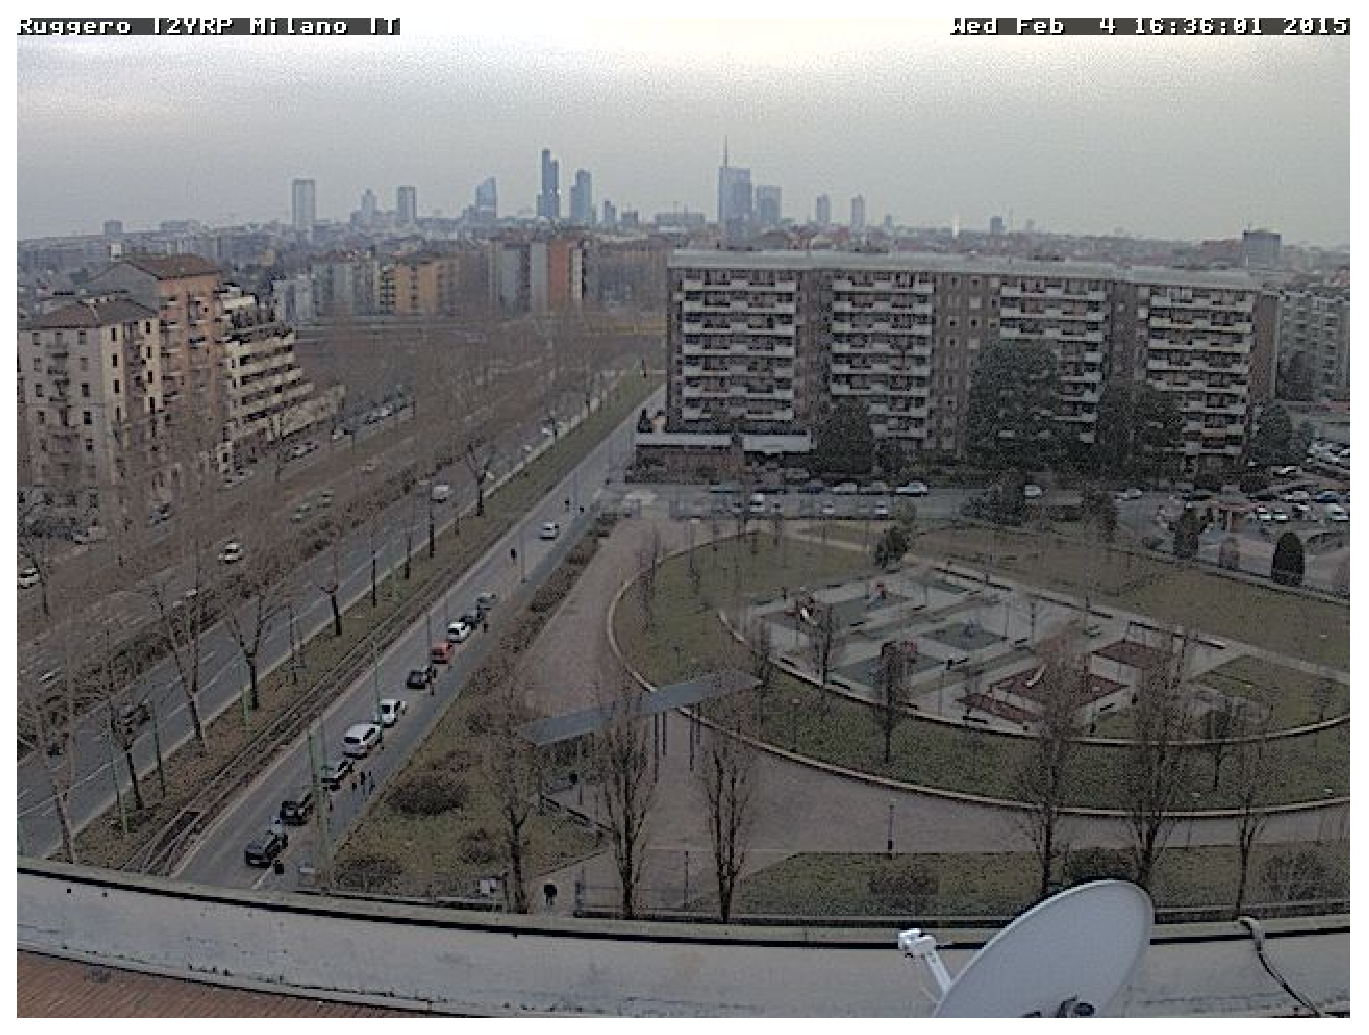
\includegraphics[width=6cm]{./pictures/testiGIORNO}}
	\end{subfigure}
	\begin{subfigure}[]
		{\label{fig:FTnotte} 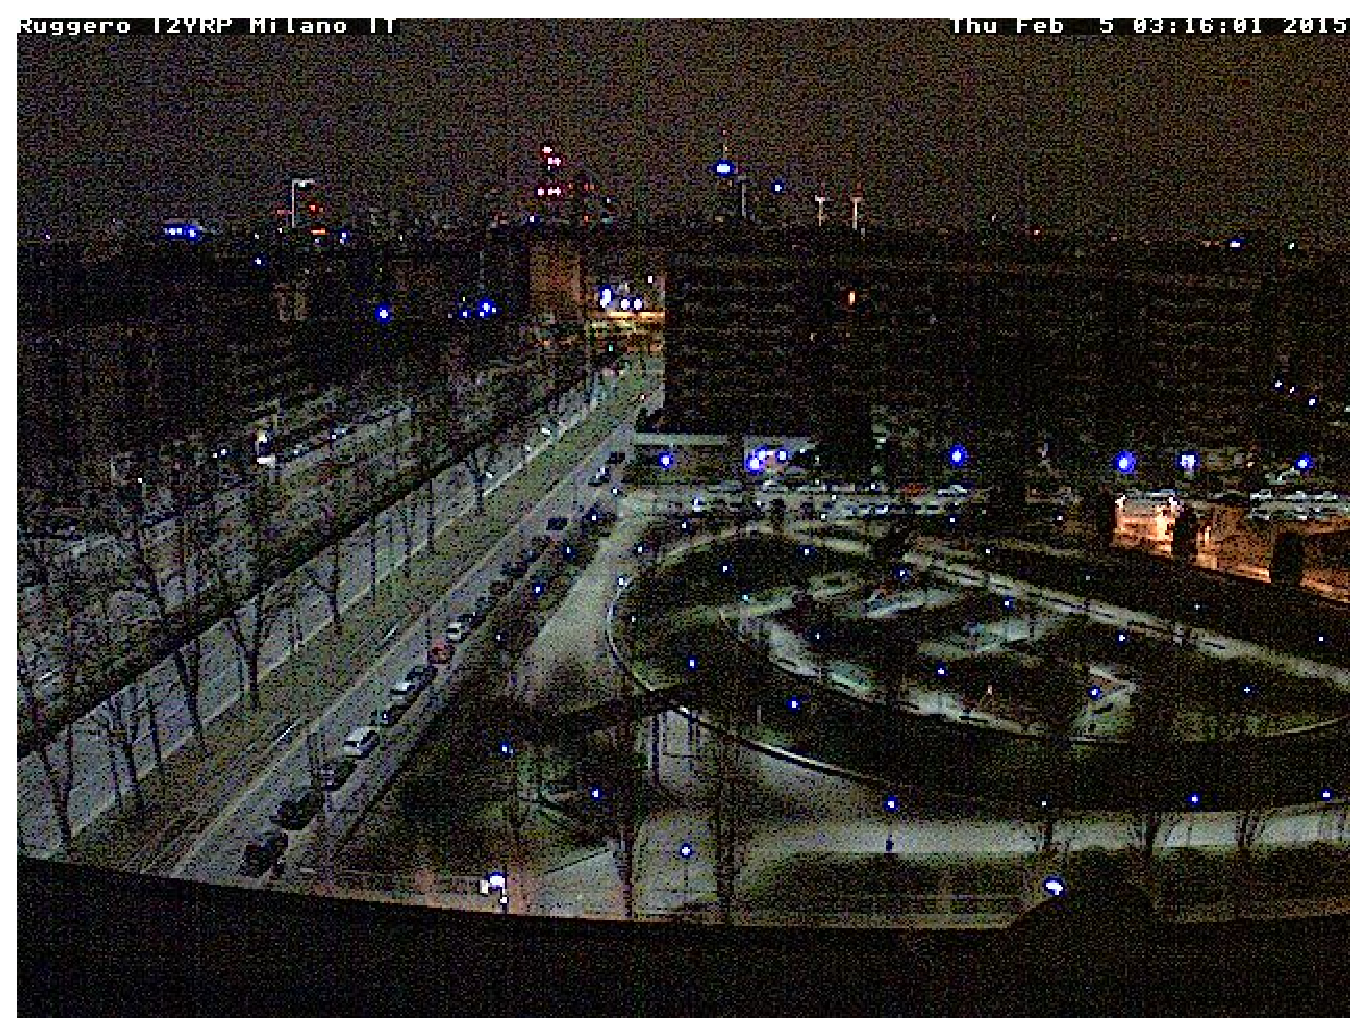
\includegraphics[width=6cm]{./pictures/testiNOTTE}}
	\end{subfigure}
	\caption[Esempio di cambi di luminosit\`a tra il giorno e la notte]{Esempio di cambi di luminosit\`a tra il giorno e la notte}
	\label{fig:testiGN}
\end{figure}
\subsection{Misura della sfocatura nell'immagine}
Nel Paragrafo \ref{sfocatura} abbiamo modellizzato il fenomeno della sfocatura secondo la formula \eqref{blur_multi}:
\[ 
z_t(x)  = \left\{ \begin{array}{lcl}
y_t(x) + \eta(x) & \mbox{per} & t < T^* \\
\mathcal{B}_t[y_t](x) + \eta(x) & \mbox{per} & t \geq T^*
\end{array}\right. , \forall x \in \mathcal{X}.
\]
Ricavare un indicatore in grado di misurare direttamente il grado di sfocatura di un'immagine \`e difficile.
Quello che \`e possibile fare, come proposto in \cite{alippi2010detecting}, \`e misurare \textit{indirettamente} il grado di sfocatura di un immagine $z_t$ basandosi sule frequenze dell'immagine.\\
Come abbiamo visto nel Paragrafo \ref{sfocatura}, l'operatore di sfocatura $\mathcal{B}$ ha come effetto principale quello di rendere le differenze di intensit\`a tra pixel adiacenti pi\`u morbide (\textit{smooth}).
In base a questa considerazione \`e possibile identificare un evento di sfocatura andando a monitorare l'\textit{energia media del gradiente} di ciascuna immagine:
\begin{equation}
	\label{eq:energyGradient}
	g(t) = \mathcal{G}[z_t] =\frac{\sum_{\mathcal{X}}\| \nabla z_t(x) \| _2^2 }{|\mathcal{X}|} ,
\end{equation}  
dove abbiamo indicato con $|\mathcal{X}|$ la \textit{cardinalit\`a} dell'insieme dei pixel $\mathcal{X}$, e con $\|\cdot\|_2$ la norma di tipo $\mathcal{L}_2$\footnote{$\|x\|_2=\sqrt{\sum_{t}x_t^2}$}.\\
Lavorando nel dominio discreto delle immagini digitali, possiamo calcolare le derivate dell'intensit\`a luminosa (\textit{luma}) per mezzo di convoluzioni con filtri derivativi.
In particolare, per il calcolo delle derivate orizzontali  abbiamo utilizzato il seguente filtro $f_h$:
\[f_h = f \circledast \left[ \begin{array}{rcl}
1 & 0 & -1
\end{array}\right], \] 
mentre per il calcolo delle derivate verticali abbiamo utilizzato il seguente filtro $f_v$:
\[f_v = f \circledast \left[ \begin{array}{r}
1 \\ 0 \\ -1
\end{array}\right], \]
dove abbiamo indicato con $\circledast$ l'operatore di convoluzione.
Il filtro $f$, invece, \`e ottenuto tramite un campionamento della \textit{funzione gaussiana} $h$, con media $0$ e deviazione standard $\sigma$
\begin{equation}
\label{eq:gaussian}
h(i,j)=\frac{1}{2\pi\sigma^2}\exp\left(-\frac{i^2+j^2}{2\sigma^2}\right),
\end{equation}
e ponendo il valore massimo di questa funzione nel centro del filtro.
Con questi filtri \`e possibile calcolare la \textit{norma del gradiente} nel seguente modo:
\begin{equation}
\label{eq:normaGradiente}
\| \nabla z_t(x) \|_2^2=\left(z_t \circledast f_h\right)(x)^2 + \left(z_t \circledast f_v\right)(x)^2.
\end{equation}
Una volta calcolata la norma del gradiente \`e possibile farne la media come specificato in \eqref{eq:energyGradient}.
Il risultato finale \`e un indicatore \textit{scalare} per ciascun frame acquisito, che pu\`o essere monitorato per individuare eventi di sfocature. 
In particolare ci aspettiamo che l'evento di sfocatura provochi un abbattimento del valore di $g$.
\subsection{Misura dello spostamento della camera}
Nel Paragrafo \ref{displacement} abbiamo modellizzato il fenomeno dello spostamento della camera secondo  \eqref{eq:displacement}
\[z_t(x)  = \left\{ \begin{array}{rcl}
y_t(x) + \eta(x) & \mbox{per} & t < T^* \\
w_t(x) + \eta(x) & \mbox{per} & t \geqslant T^*
\end{array}\right. , \forall x \in \mathcal{X}\]
dove $T^*$ indica l'istante in cui avviene il cambiamento.\\
Uno spostamento della camera, quindi, pu\`o essere rilevato come un cambiamento \textit{globale} dei valori di intensit\`a luminosa (\textit{luma}) nei pixel dell'immagine.
\begin{figure}[tb]
	\centering
	\begin{subfigure}[]
		{\label{fig:BAgiorno} 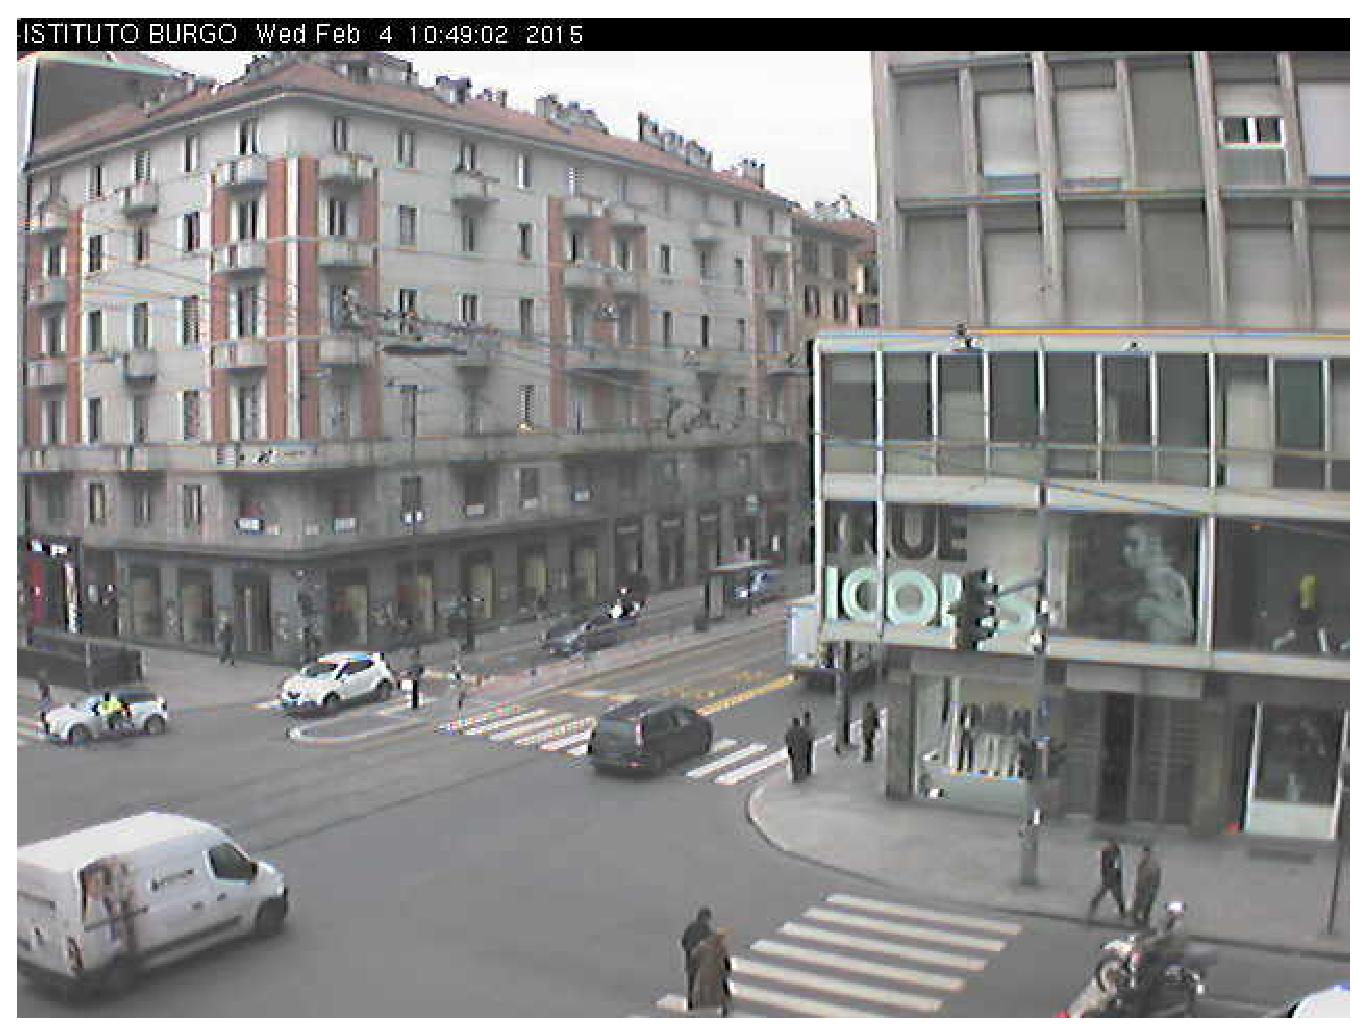
\includegraphics[width=6cm]{./pictures/buenosAiresGIORNO}}
	\end{subfigure}
	\begin{subfigure}[]
		{\label{fig:BAnotte} 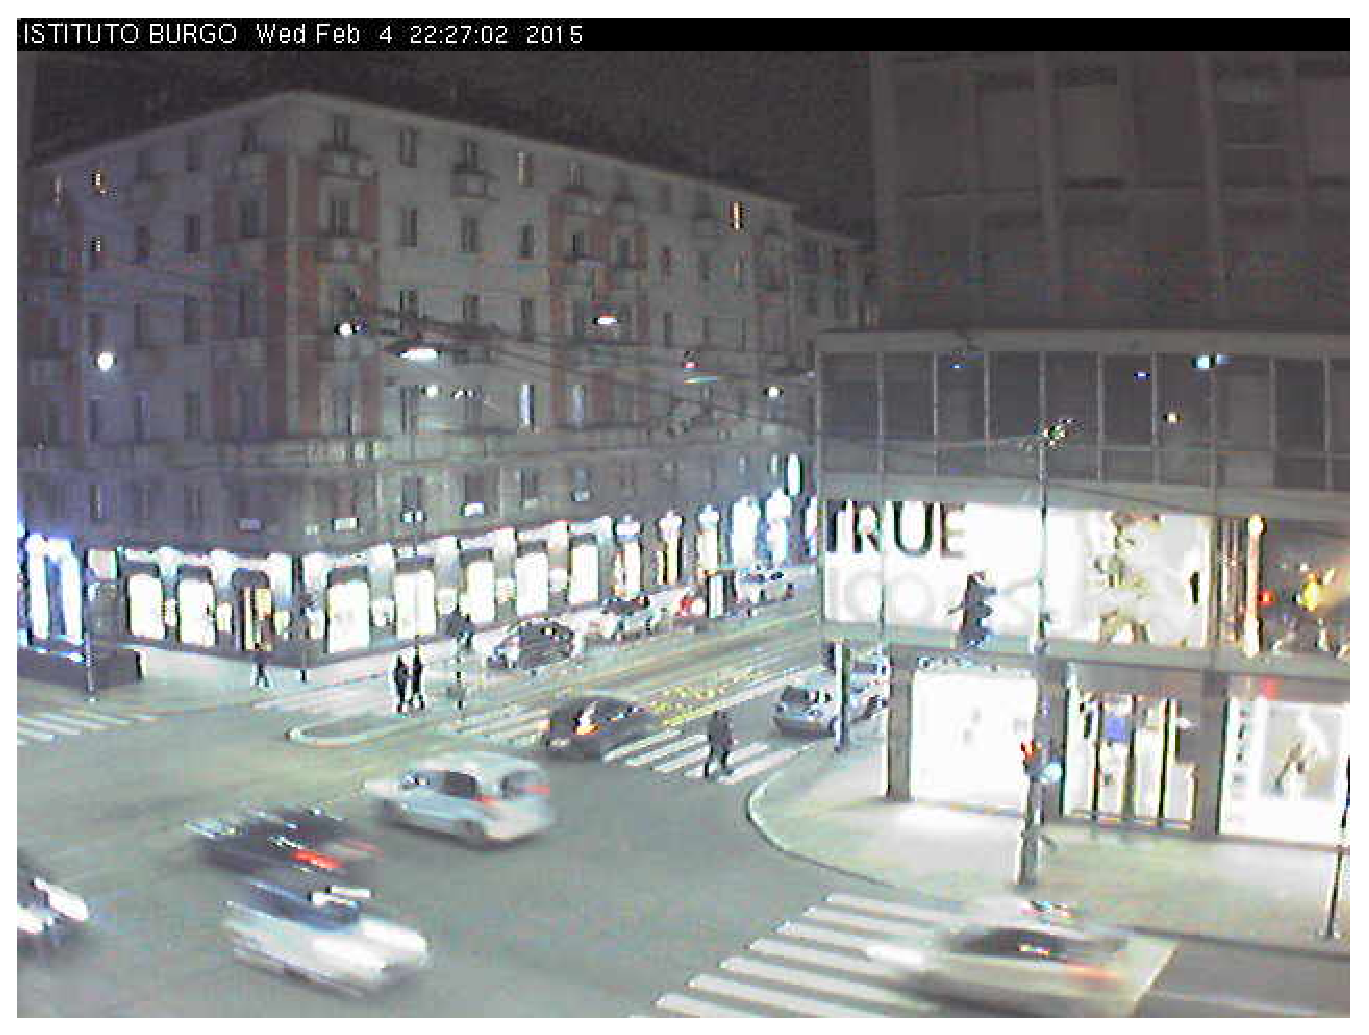
\includegraphics[width=6cm]{./pictures/buenosAiresNOTTE}}
	\end{subfigure}
	\caption[Esempio di presenza di sfocature dovute all'aumento del tempo di esposizione della camera]{In questo esempio vediamo come l'aumentare il tempo di esposizione della camera porti come effetto una presenza di sfocature nelle zone dove sono presenti oggetti in movimento. 
		In (a), dove il frame \`e acquisito durante il giorno, vediamo come le macchine in movimento siano riprese in maniera nitida, mentre in (b), dove il frame \`e ripreso durante la notte, le zone con le macchine risultano sfocate.}
	\label{fig:buenosAiresGN}
\end{figure}
\begin{figure}[tbp]
	\centering
	\begin{subfigure}[]
		{\label{fig:collage} \includegraphics[width=12cm]{./pictures/buenosAiresCollage}}
	\end{subfigure}
	\begin{subfigure}[]
		{\label{fig:energy} 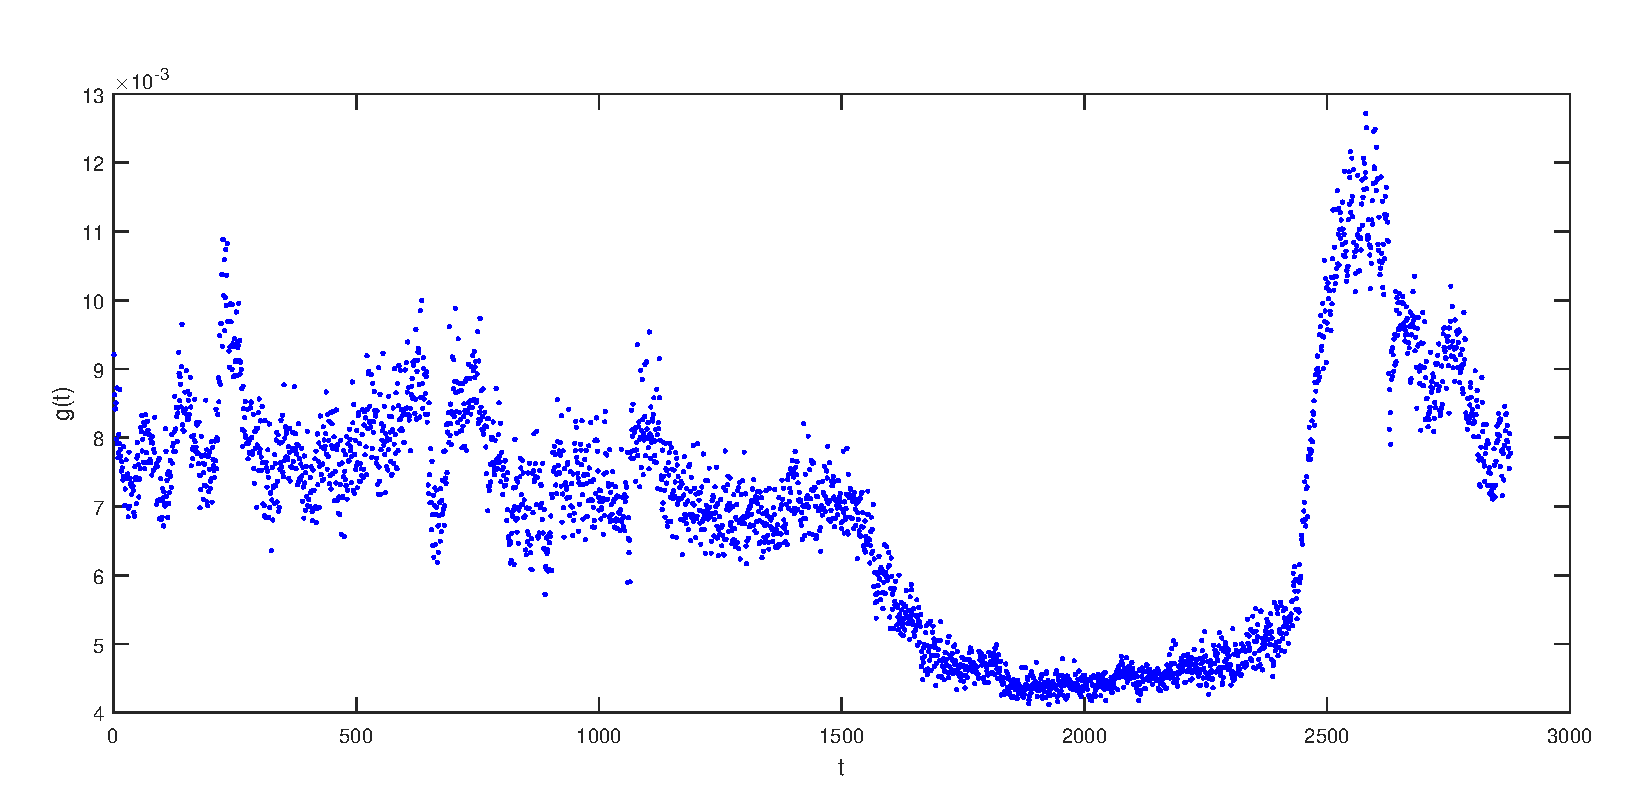
\includegraphics[width=12cm]{./pictures/energyTot}}
	\end{subfigure}
	\begin{subfigure}[]
		{\label{fig:energyDetr} 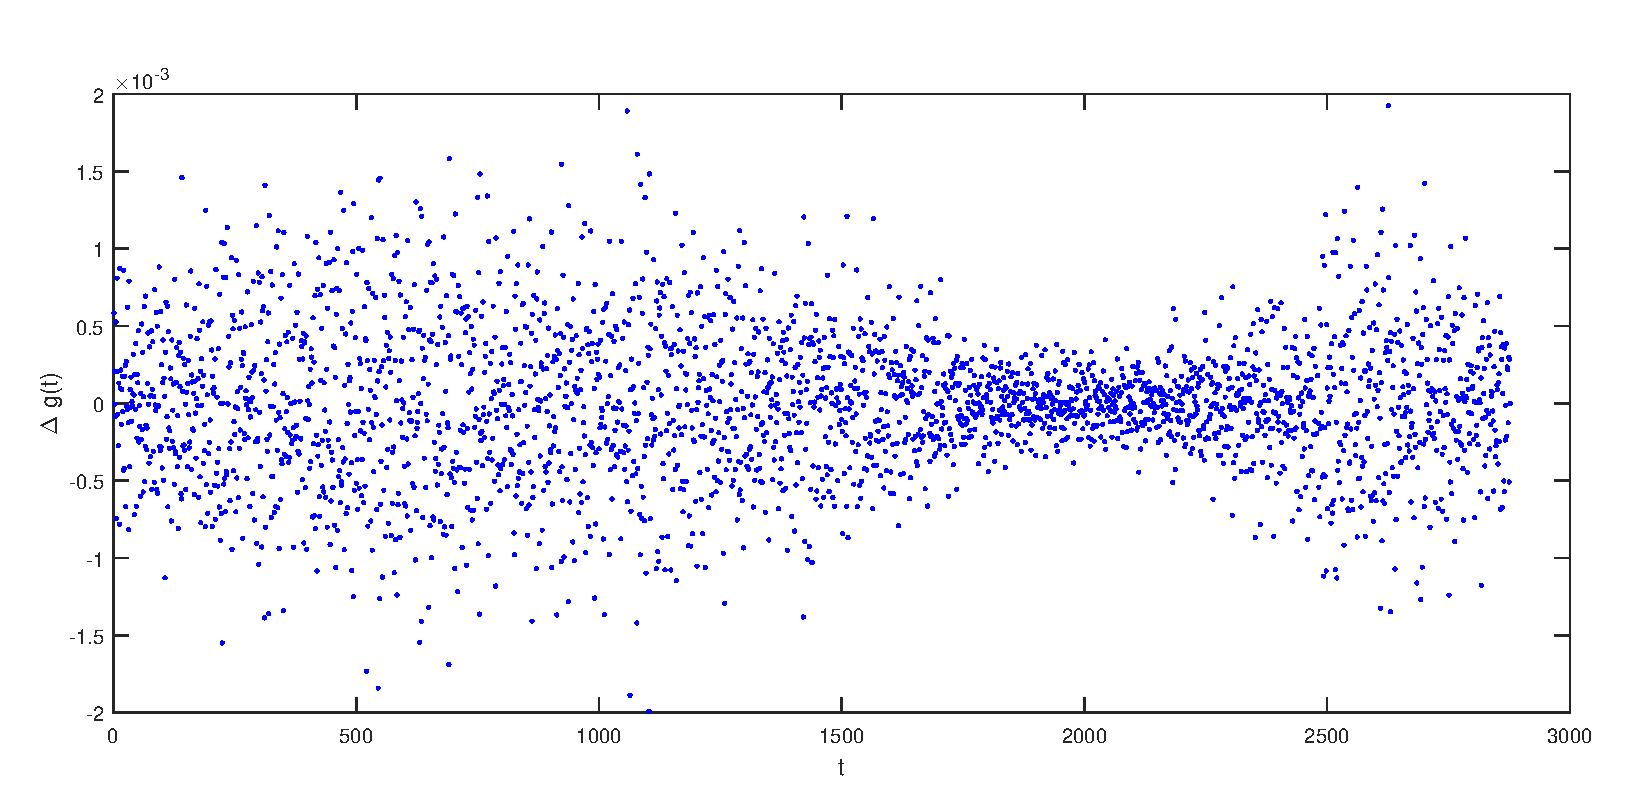
\includegraphics[width=12cm]{./pictures/energydetr}}
	\end{subfigure}
	\caption[Energia media del gradiente lungo un'acquisizione di 24 ore e suo detrending]
	{In questo esempio vediamo il comportamento dell'energia media del gradiente su una sequenza di 24 ore in cui non avvengono eventi di tampering.
		In (a) sono riportati alcuni frame estratti dalla sequenza.
		In (b) vediamo il comportamento dell'indicatore $g(t)$, e in (c) quello del suo detrending .
		Anche in assenza di tampering, l'indicatore $g(t)$ presenta un andamento molto irregolare e difficilmente prevedibile.
		Il detrending dell'indicatore, invece, possiede un andamento pi\`u stazionario, incentrato sul valore $0$.
	}
	\label{fig:energyTot}
\end{figure}
%\clearpage
%\cleartoevenpage
\begin{figure}[tbp]
	\centering
	\begin{subfigure}[]
		{\label{fig:collage2} \includegraphics[width=12cm]{./pictures/buenosAiresCollage}}
	\end{subfigure}
	\begin{subfigure}[]
		{\label{fig:luma} 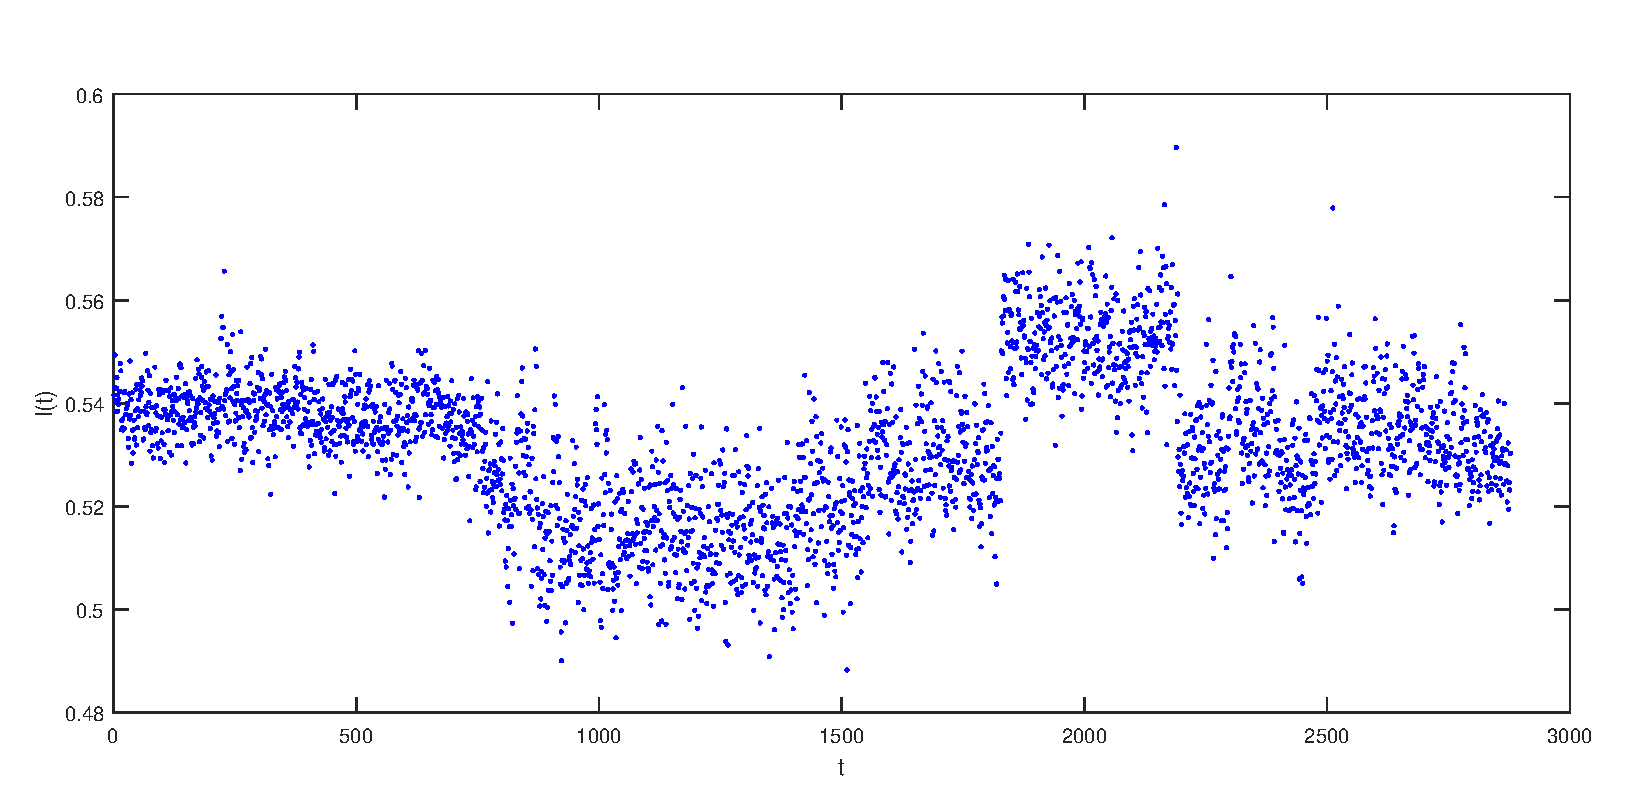
\includegraphics[width=12cm]{./pictures/lumaTot}}
	\end{subfigure}
	\begin{subfigure}[]
		{\label{fig:lumaDetr} 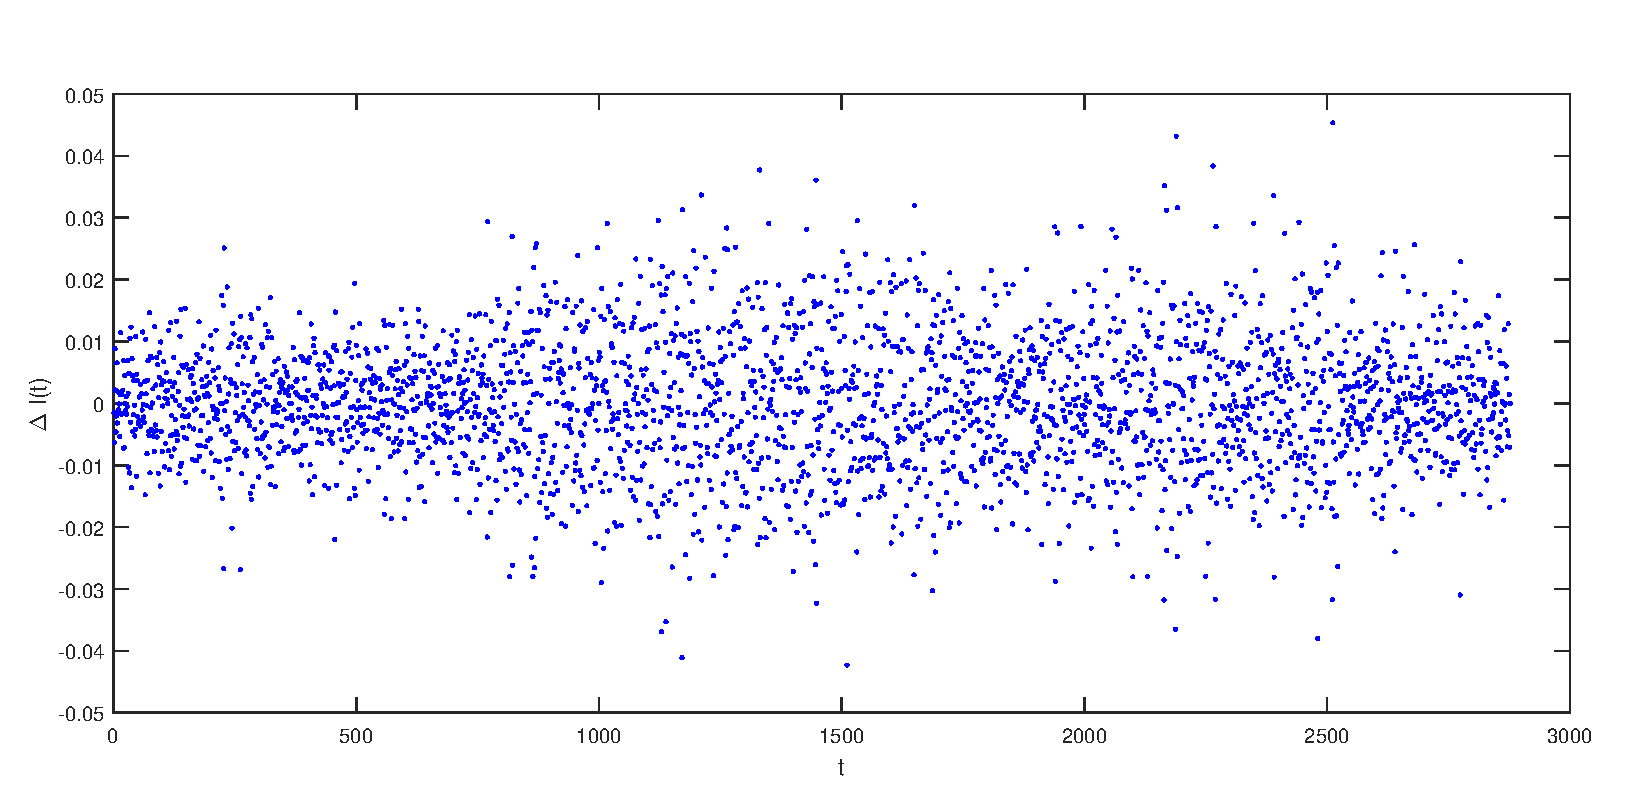
\includegraphics[width=12cm]{./pictures/lumadetr}}
	\end{subfigure}
	\caption[Energia media della luma lungo un'acquisizione di 24 ore e suo detrending]
	{In questo esempio vediamo il comportamento dell'energia media della luma su una sequenza di 24 ore in cui non avvengono eventi di tampering.
		In (a) sono riportati alcuni frame estratti dalla sequenza.
		In (b) vediamo il comportamento dell'indicatore $l(t)$, e in (c) quello del suo detrending .
		Anche in assenza di tampering, l'indicatore $l(t)$ presenta un andamento molto irregolare e difficilmente prevedibile.
		Il detrending dell'indicatore, invece, possiede un andamento pi\`u stazionario, incentrato sul valore $0$.
	}
	\label{fig:lumaTot}
\end{figure}
In base a questo \`e possibile identificare un evento di spostamento della camera andando a monitorare l'\textit{energia media della luma} di ciascuna immagine:
\begin{equation}
\label{eq:energyLuma}
l(t) = \mathcal{L}[z_t] =\frac{\sum_{\mathcal{X}} z_t(x) }{|\mathcal{X}|} ,
\end{equation}  
dove abbiamo indicato con $|\mathcal{X}|$ la \textit{cardinalit\`a} dell'insieme dei pixel $\mathcal{X}$.\\
Il risultato finale \`e un indicatore \textit{scalare} per ciascun frame acquisito, che pu\`o essere monitorato per individuare eventi di spostamenti della camera. 
\subsection{Comportamento degli indicatori nel tempo}
\label{comportamento}
Analizzando alcune sequenze video abbiamo notato che, anche in assenza di eventi di tampering, vi sono alcuni fattori che sono in grado di far variare il valore degli indicatori estratti.
Tra i pi\`u importanti abbiamo:
\begin{itemize}
	\item \textit{Cambiamenti di luminosit\`a} che avvengono nel corso della giornata. 
	Se consideriamo l'esempio in Figura \ref{fig:testiGN}, possiamo notare come, nel passaggio dal giorno (Figura \ref{fig:FTgiorno}) alla notte (Figura \ref{fig:FTnotte}), le differenze di luminosit\`a siano elevate.  
	\item \textit{Dinamicit\`a della scena}. La ripresa di una scena dinamica, come ad esempio una strada, ha come risultato che ciascun frame sia diverso dagli altri.
	Ci\`o si traduce in una variabilit\`a elevata degli indicatori che abbiamo utilizzato. 
	Inoltre, col passare del tempo, pu\`o succedere che cambi anche il \textit{grado di dinamicit\`a} della scena.
	Considerando ancora l'esempio della strada avremo dei momenti in cui il traffico \`e pi\`u intenso (nelle cosiddette \textit{ore di punta}) e altri in cui le macchine passano meno spesso (tipicamente durante la notte).
	\item \textit{Tempo di esposizione della camera}. Solitamente le camere sono in grado di configurare in maniera automatica alcuni parametri che regolano l'acquisizione dell'immagine, in base alle condizioni di luminosit\`a esterne.
	Ad esempio, durante la ripresa di scene notturne la camera solitamente aumenta il \textit{tempo di esposizione} del sensore, in modo che esso possa ricevere pi\`u luce possibile.
	Ci\`o porta alla \textit{presenza di sfocature} nel caso vengano immortalati degli oggetti in movimento (come ad esempio le macchine che si muovono nella Figura \ref{fig:BAnotte}).
	Nel caso in cui il tempo di esposizione non fosse sufficiente, invece, i cambiamenti di luminosit\`a potrebbero portare a un aumento del rumore nei frame acquisiti nelle ore pi\`u scure, in quanto il sensore riceverebbe meno luce.
\end{itemize} 
%\cleartoevenpage
%\clearpage
Questi fenomeni fanno s\`i che i nostri indicatori abbiano una dinamica \textit{difficilmente prevedibile} e che \textit{non siano stazionari}\footnote{Ovvero non sono realizzazioni i.i.d. di una stessa variabile aleatoria}, come possiamo vedere dal comportamento dell'energia del gradiente nella Figura \ref{fig:energy} e da quello dell'energia media della luma nella Figura \ref{fig:luma}.
I due grafici riportano l'andamento degli indicatori durante una ripresa di $24$ ore, acquisendo un frame ogni minuto, in cui non sono avvenuti eventi di tampering.
Il fatto che questi indicatori non si comportino in maniera stazionare anche nel caso in cui non avvengano eventi di tampering rende impossibile applicare direttamente le tecniche di CDT come in \cite{alippi2010detecting}. \\
\subsection{Detrending degli indicatori}
Osservando l'andamento degli indicatori nelle Figure \ref{fig:energy} e \ref{fig:luma} possiamo notare la presenza di componenti ad alta frequenza, dovute dal rumore nelle immagini, e di componenti in bassa frequenza, dovute prevalentemente ai cambi di luce e dalla dinamicit\`a della scena.
Per eliminare le componenti in bassa frequenza, che sono quelle che rendono i nostri indicatori non prevedibili, possiamo fare un \textit{detrending} di ciascun segnale calcolando la \textit{differenza} tra l'indicatore all'istante corrente e quello precedente.
Nel caso dell'energia media del gradiente avremo
\begin{equation}
\label{eq:gradientDetr}
\frac{\partial g}{\partial t}(t) = g(t) - g(t-1),
\end{equation}
mentre per l'energia media della luma avremo
\begin{equation}
\label{eq:lumaDetr}
\frac{\partial l}{\partial t}(t) = l(t) - l(t-1).
\end{equation}
Vediamo un esempio di come si comporta il detrending sui nostri indicatori nelle Figure \ref{fig:energyDetr} e \ref{fig:lumaDetr}.  
%\cleartoevenpage
\begin{figure}[tbp]
	\centering
	\begin{subfigure}[]
		{\label{fig:collage3} \includegraphics[width=12cm]{./pictures/buenosAiresCollageDefocus}}
	\end{subfigure}
	\begin{subfigure}[]
		{\label{fig:energyDefocus} 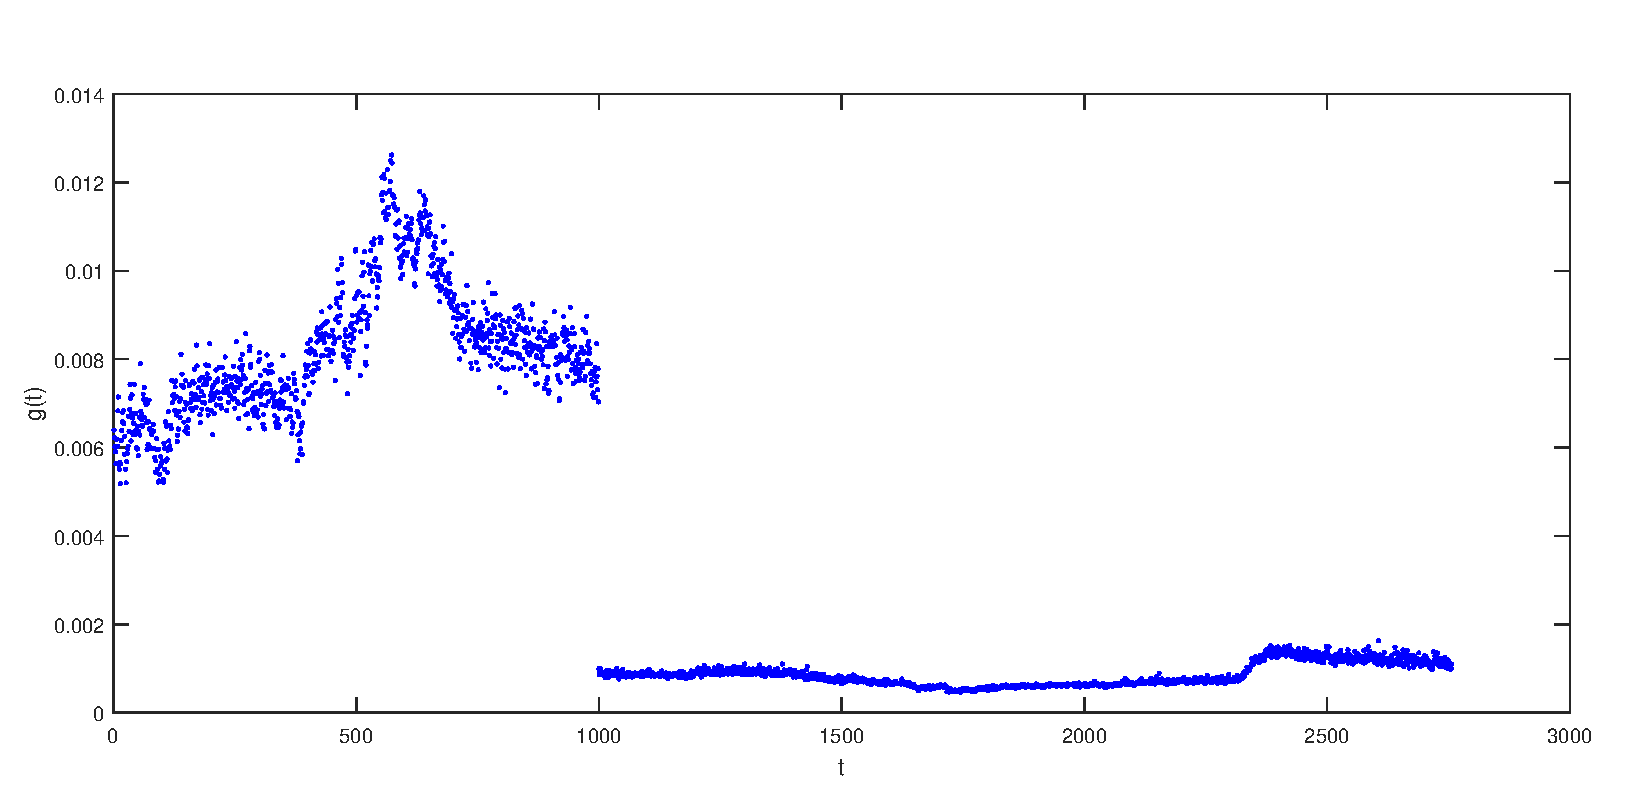
\includegraphics[width=12cm]{./pictures/Defocus/DEFOCUS_energy}}
	\end{subfigure}
	\begin{subfigure}[]
		{\label{fig:energyDetrDefocus} 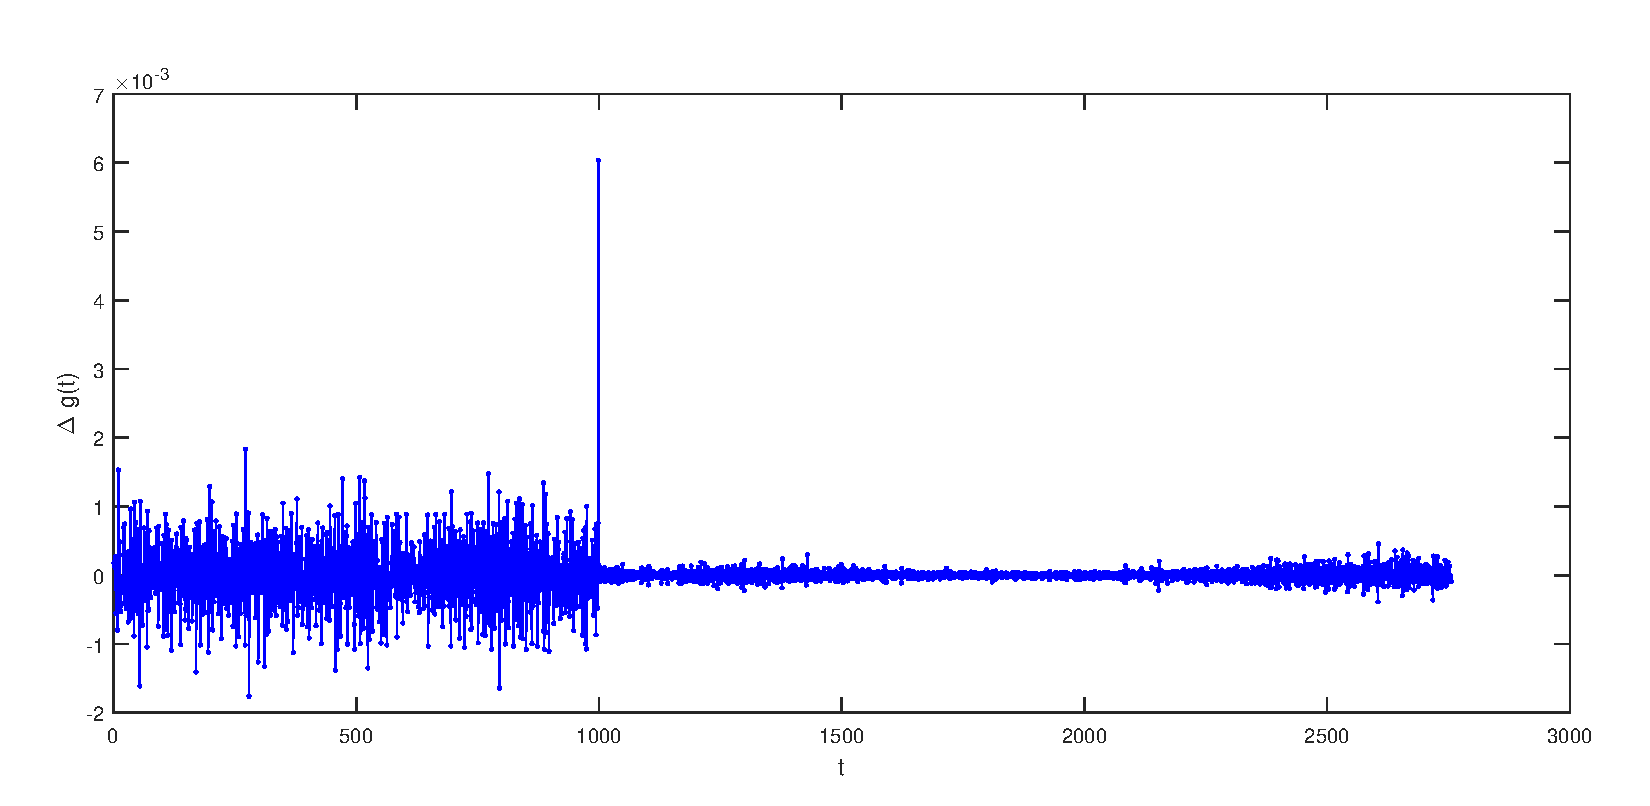
\includegraphics[width=12cm]{./pictures/Defocus/DEFOCUS_energy_detr}}
	\end{subfigure}
	\caption[Energia media del gradiente e suo detrending nel caso di una sfocatura]
	{In questo esempio vediamo il comportamento dell'energia media del gradiente su una sequenza di 24 ore in cui avviene un evento di sfocatura.
		In (a) sono riportati alcuni frame estratti dalla sequenza. 
		La sfocatura avviene al frame $1000$ e continua per il resto della sequenza.
		In (b) vediamo il comportamento dell'indicatore $g(t)$, e in (c) quello del suo detrending.
		Vediamo come in (b) l'evento di sfocatura si traduca in un crollo del valore di $g(t)$.
		In (c), invece, vediamo che l'evento si traduce in un picco nel valore del detrending nell'istante in cui inizia la sfocatura, e in una diminuzione della varianza negli istanti successivi}
	\label{fig:defocusPLOT}
\end{figure}
%%\clearpage
%\cleartoevenpage
\begin{figure}[tbp]
	\centering
	\begin{subfigure}[]
		{\label{fig:collage4} \includegraphics[width=12cm]{./pictures/buenosAiresCollageDefocus}}
	\end{subfigure}
	\begin{subfigure}[]
		{\label{fig:lumaDefocus} 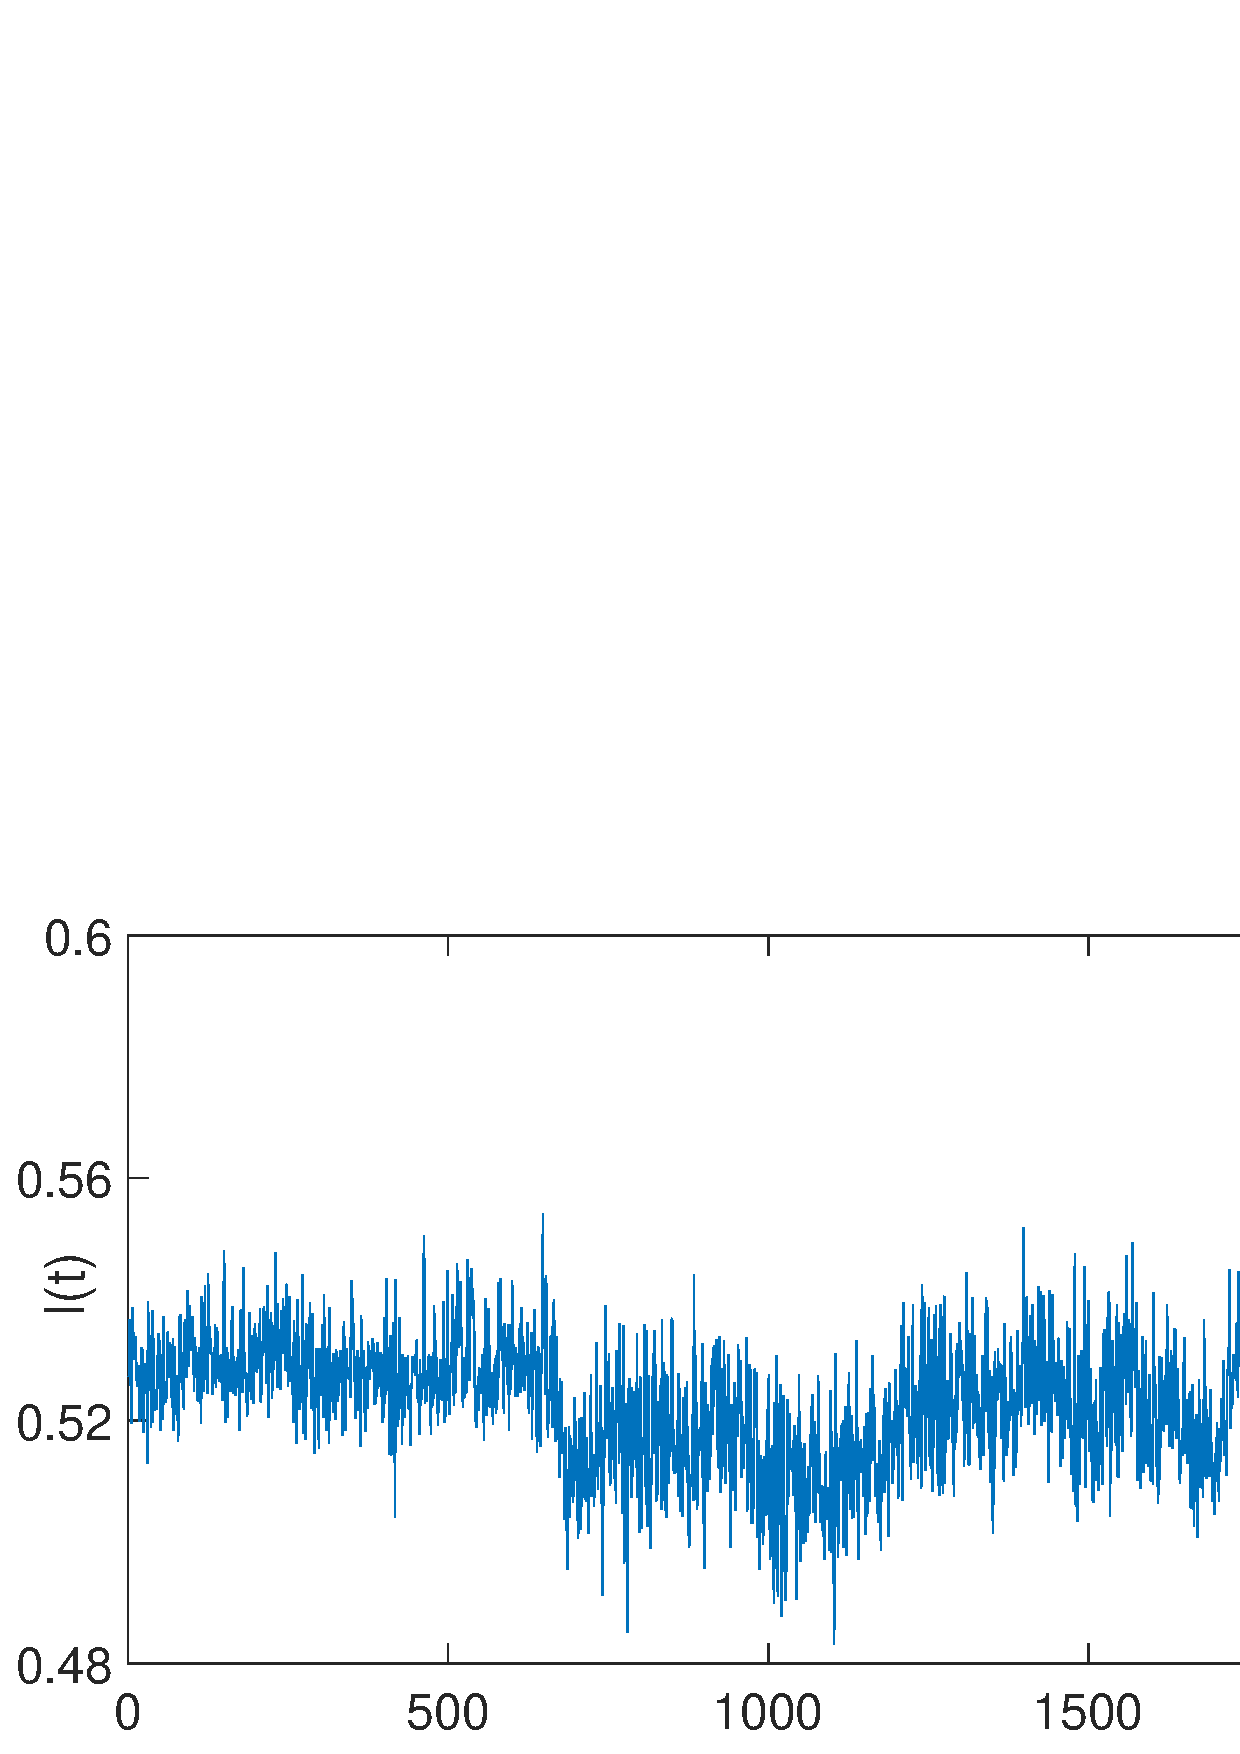
\includegraphics[width=12cm]{./pictures/Defocus/DEFOCUS_luma}}
	\end{subfigure}
	\begin{subfigure}[]
		{\label{fig:lumaDetrDefocus} 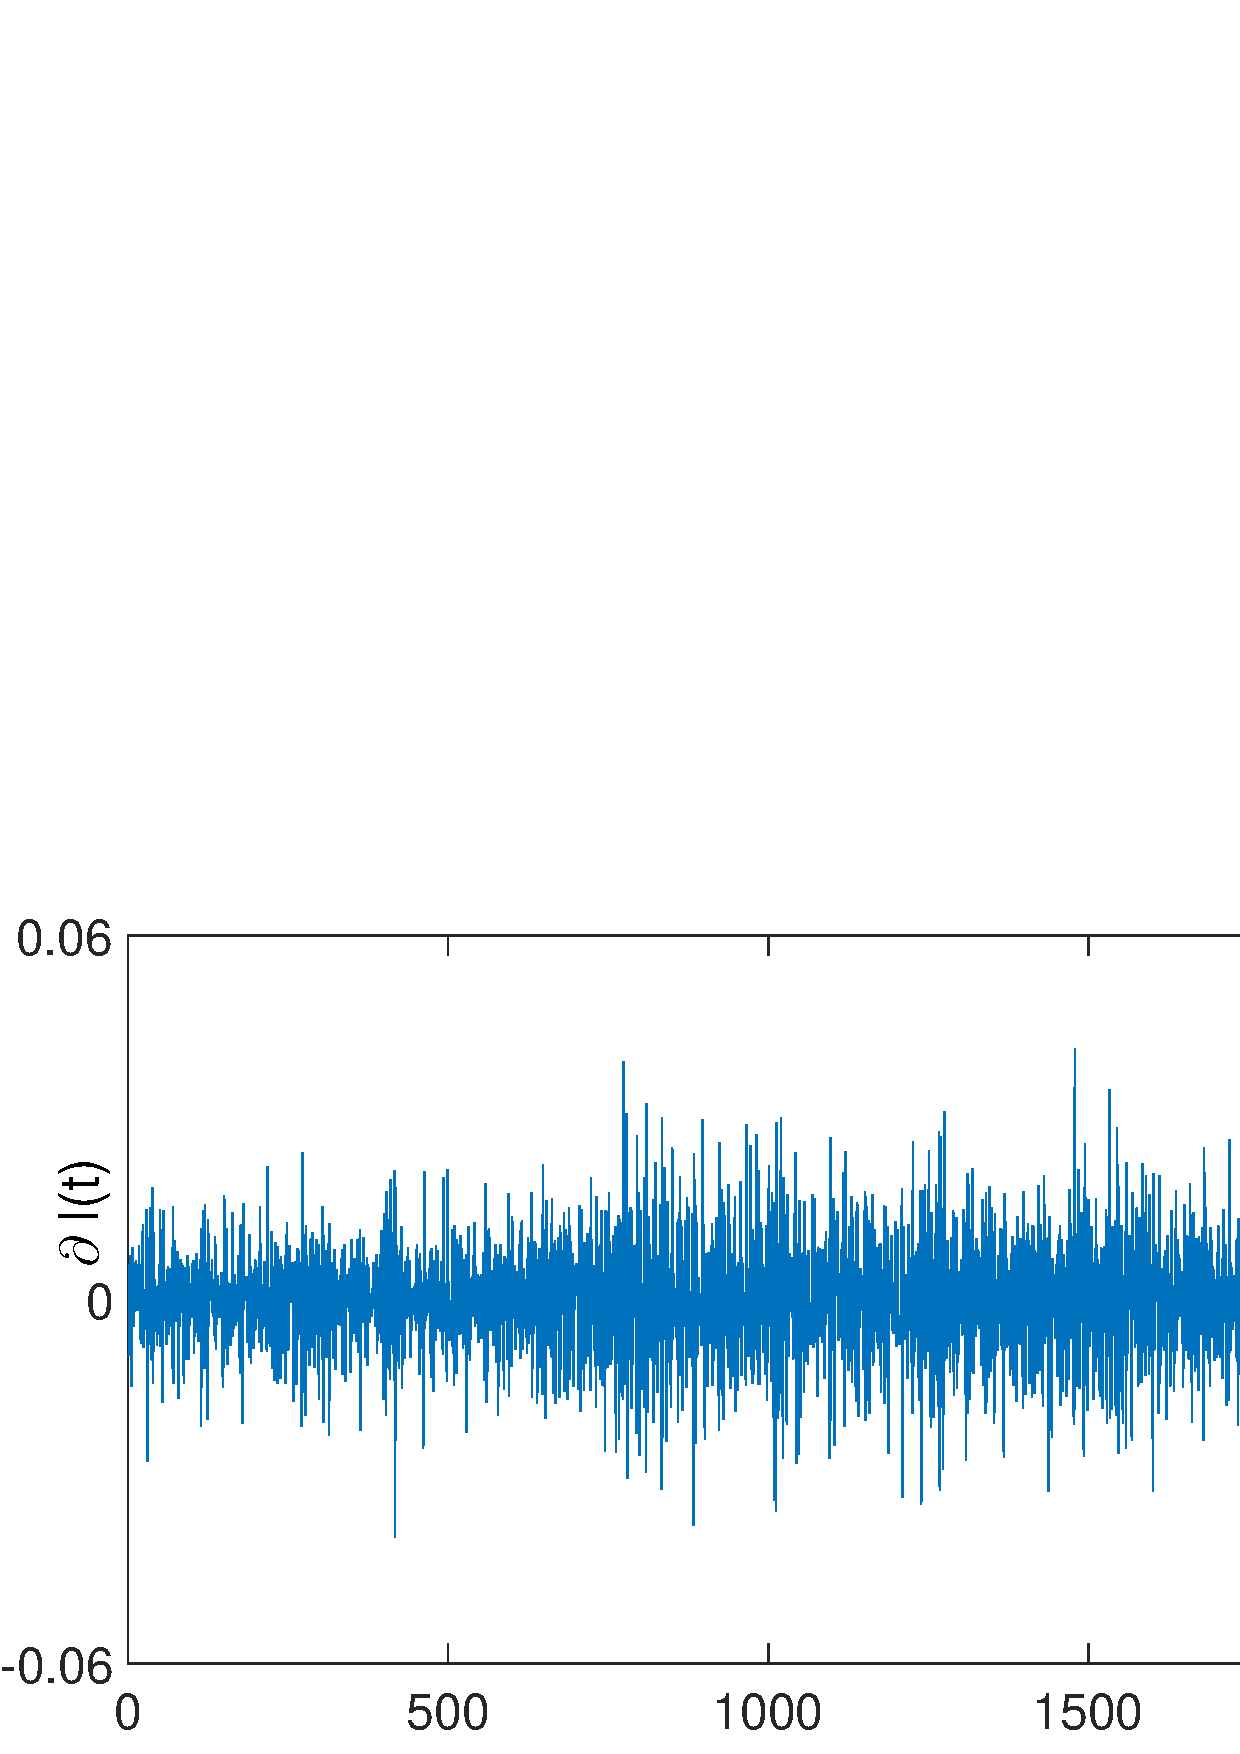
\includegraphics[width=12cm]{./pictures/Defocus/DEFOCUS_luma_detr}}
	\end{subfigure}
	\caption[Energia media della luma e suo detrending nel caso di una sfocatura]
	{In questo esempio vediamo il comportamento dell'energia media della luma su una sequenza di 24 ore in cui avviene un evento di sfocatura.
		In (a) sono riportati alcuni frame estratti dalla sequenza. 
		La sfocatura avviene al frame $1000$ e continua per il resto della sequenza.
		Vediamo come il comportamento dell'indicatore $l(t)$ (b) e quello del suo detrending (c) non siano influenzati dall'evento di sfocatura.
		Questo avviene perch\'e questo tipo di tampering abbatte le alte frequenze presenti nell'immagine, mantenendo comunque il valore medio della luma invariato.
		}
	\label{fig:defocusDetrPLOt}
\end{figure}
%%\clearpage
Possiamo notare come le fluttuazioni in bassa frequenza vengano rimosse dal detrending, visto che gli indicatori di due frame consecutivi sono pressoch\'e costanti.\\
Come abbiamo detto prima, lo scopo del monitoraggio di questi indicatori \`e quello di individuare degli eventi di tampering.
Nelle Figure \ref{fig:defocusPLOT} e \ref{fig:displacementPLOT} possiamo vedere il comportamento dell'energia media di luma e gradiente rispettivamente per un caso di sfocatura e per un caso di spostamento della camera.  
In particolare, in entrambi i casi l'evento di tampering avviene al frame $1000$\footnote{Il modo in cui sono stati ottenuti gli eventi di tampering \`e descritto nel Capitolo \ref{ProveSperimentali}}.
Il detrending di questi segnali \`e visualizzato nelle Figure \ref{fig:defocusDetrPLOt} e \ref{fig:displacementDetrPLOT}.\\
%\cleartoevenpage
\begin{figure}[tbp]
	\centering
	\begin{subfigure}[]
		{\label{fig:collage5} \includegraphics[width=12cm]{./pictures/buenosAiresCollageDisplacement}}
	\end{subfigure}
	\begin{subfigure}[]
		{\label{fig:energyDisplacement} 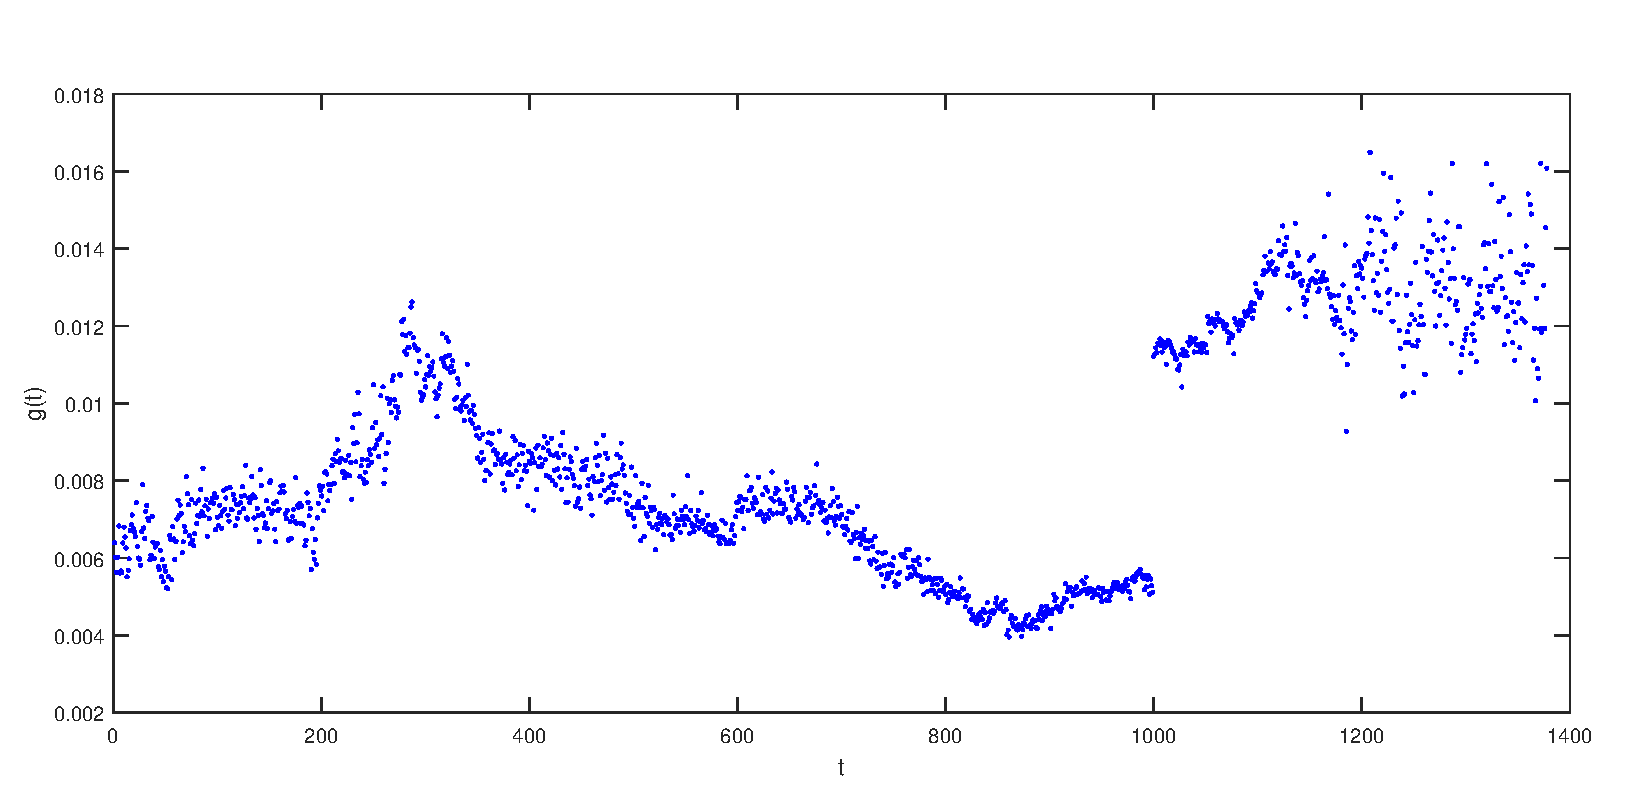
\includegraphics[width=12cm]{./pictures/Displacement/DISPLACEMENT_energy}}
	\end{subfigure}
	\begin{subfigure}[]
		{\label{fig:energyDetrDisplacement} 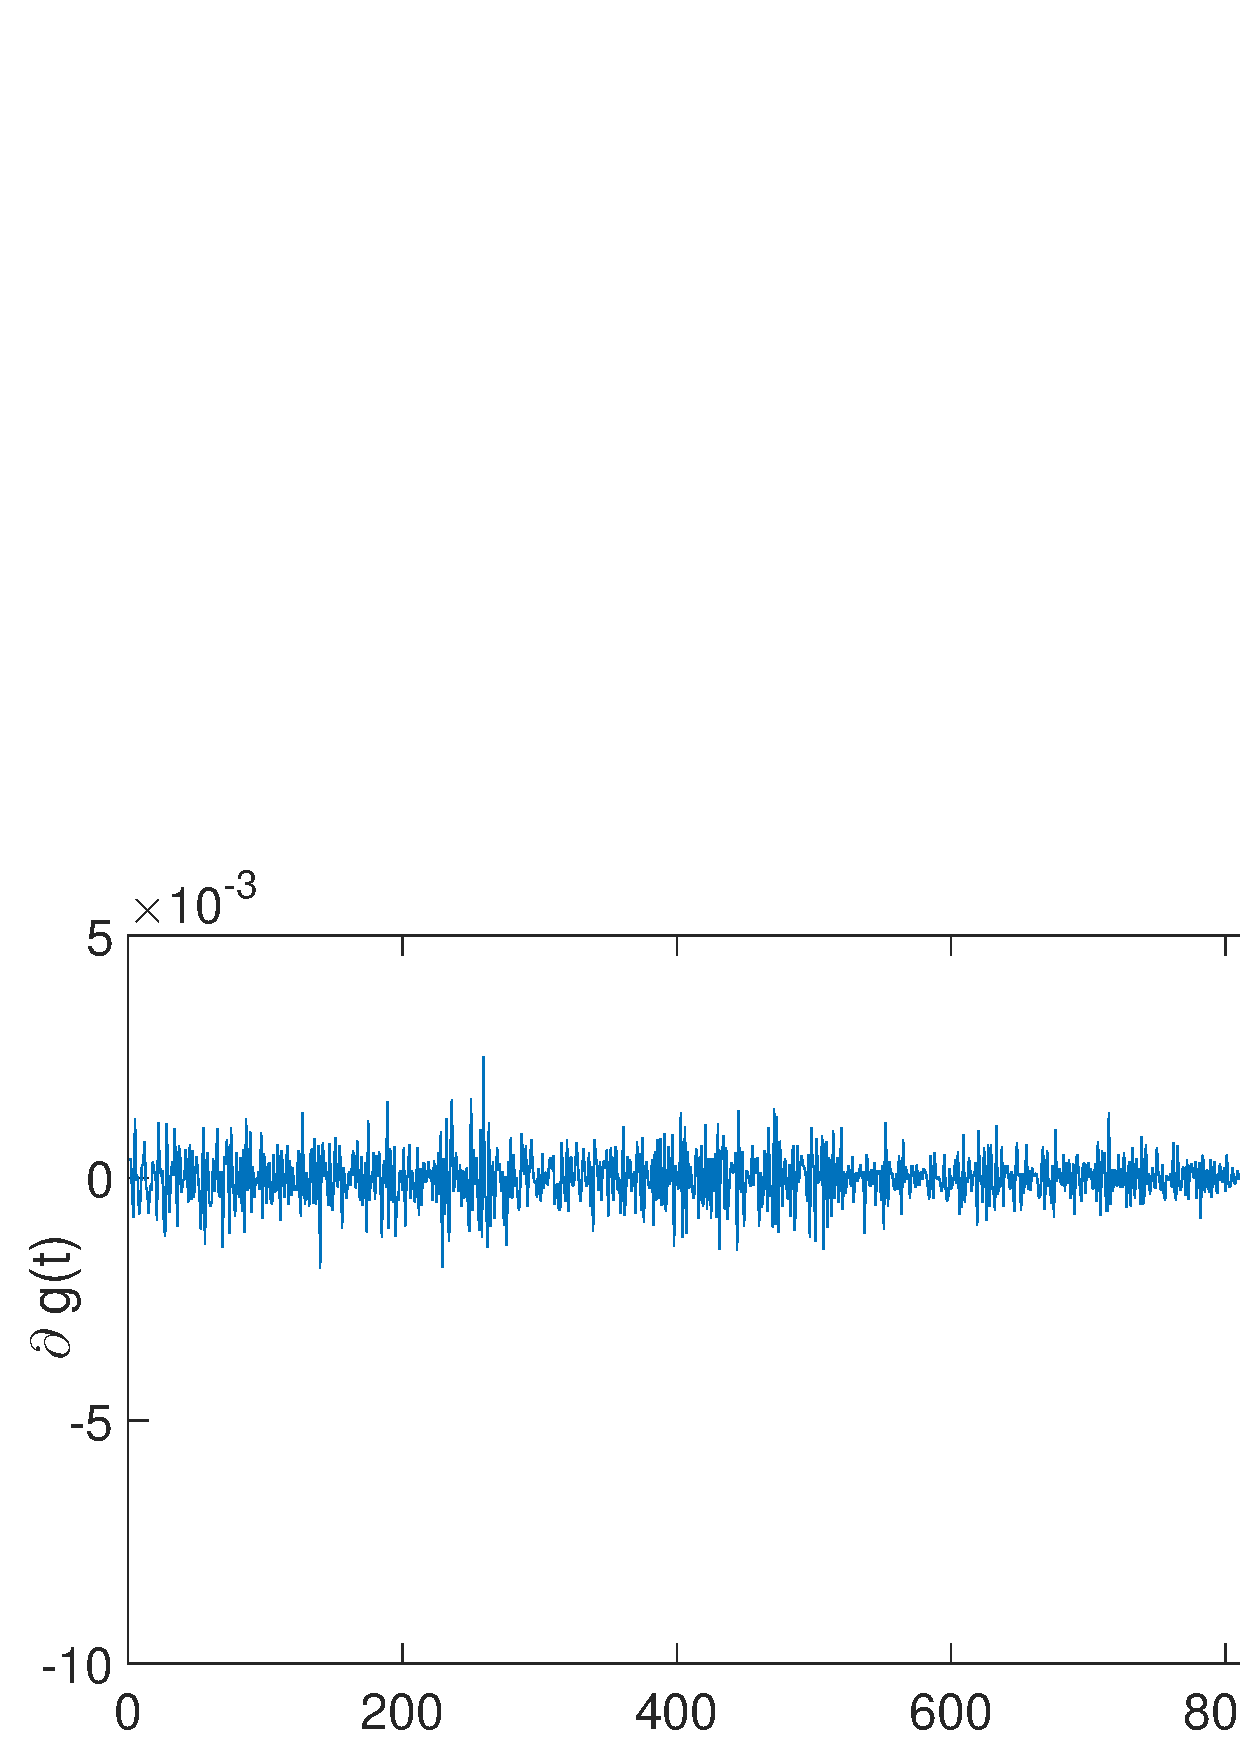
\includegraphics[width=12cm]{./pictures/Displacement/DISPLACEMENT_energy_detr}}
	\end{subfigure}
	\caption[Energia media del gradiente e suo detrending nel caso di uno spostamento della camera]
	{In questo esempio vediamo il comportamento dell'energia media del gradiente su una sequenza di 24 ore in cui avviene un evento di spostamento della camera.
		In (a) sono riportati alcuni frame estratti dalla sequenza. 
		Lo spostamento della camera avviene al frame $1000$ e, per il resto della sequenza, l'inquadratura rimane la stessa.
		In (b) vediamo il comportamento dell'indicatore $g(t)$, e in (c) quello del suo detrending.
		Vediamo come in (b) l'evento di spostamento della camera si traduca in un salto del valore di $g(t)$.
		In (c), invece, vediamo che l'evento si traduce in un picco (in questo caso negativo) nel valore del detrending nell'istante in cui inizia la sfocatura.}
	\label{fig:displacementPLOT}
\end{figure}
%%\clearpage
%\cleartoevenpage
\begin{figure}[tbp]
	\centering
	\begin{subfigure}[]
		{\label{fig:collage6} \includegraphics[width=12cm]{./pictures/buenosAiresCollageDisplacement}}
	\end{subfigure}
	\begin{subfigure}[]
		{\label{fig:lumaDisplacement} 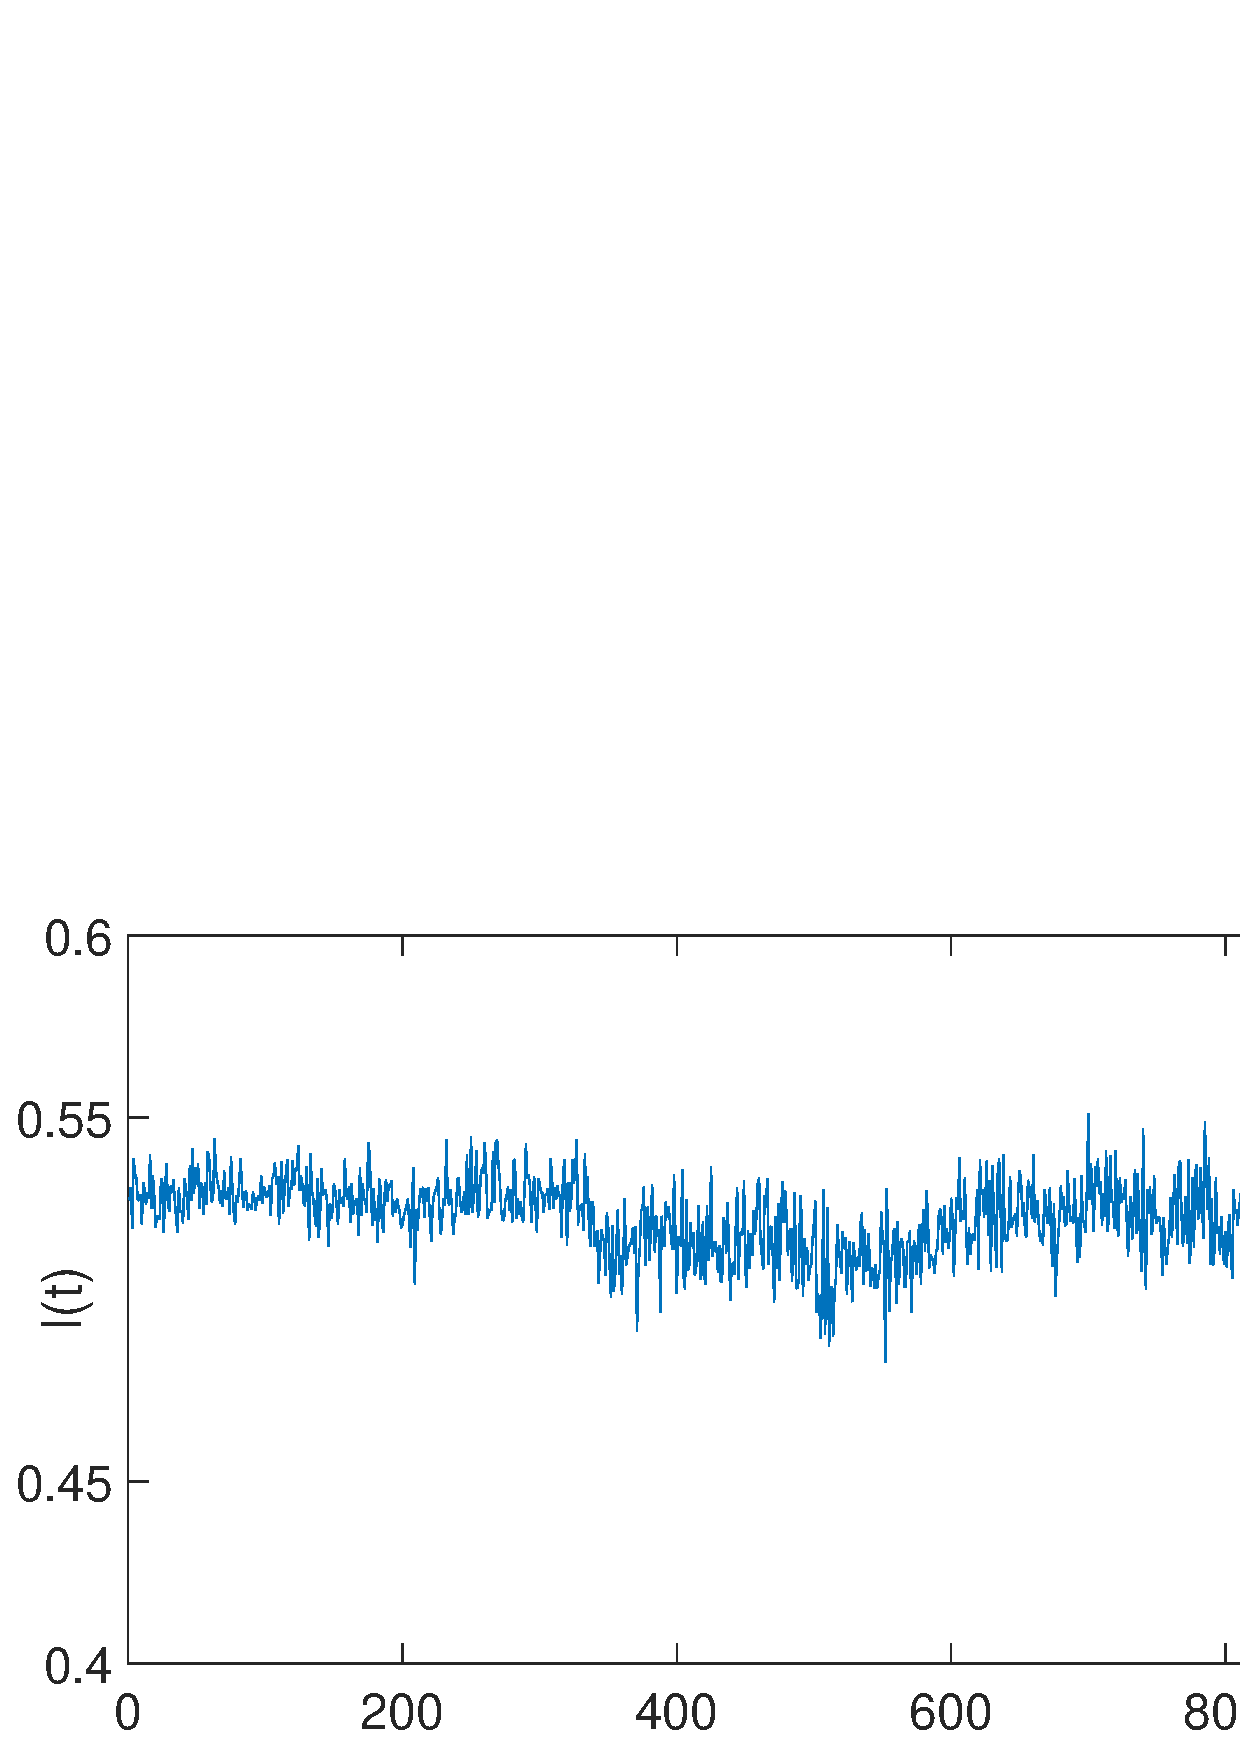
\includegraphics[width=12cm]{./pictures/Displacement/DISPLACEMENT_luma}}
	\end{subfigure}
	\begin{subfigure}[]
		{\label{fig:lumaDetrDisplacement} 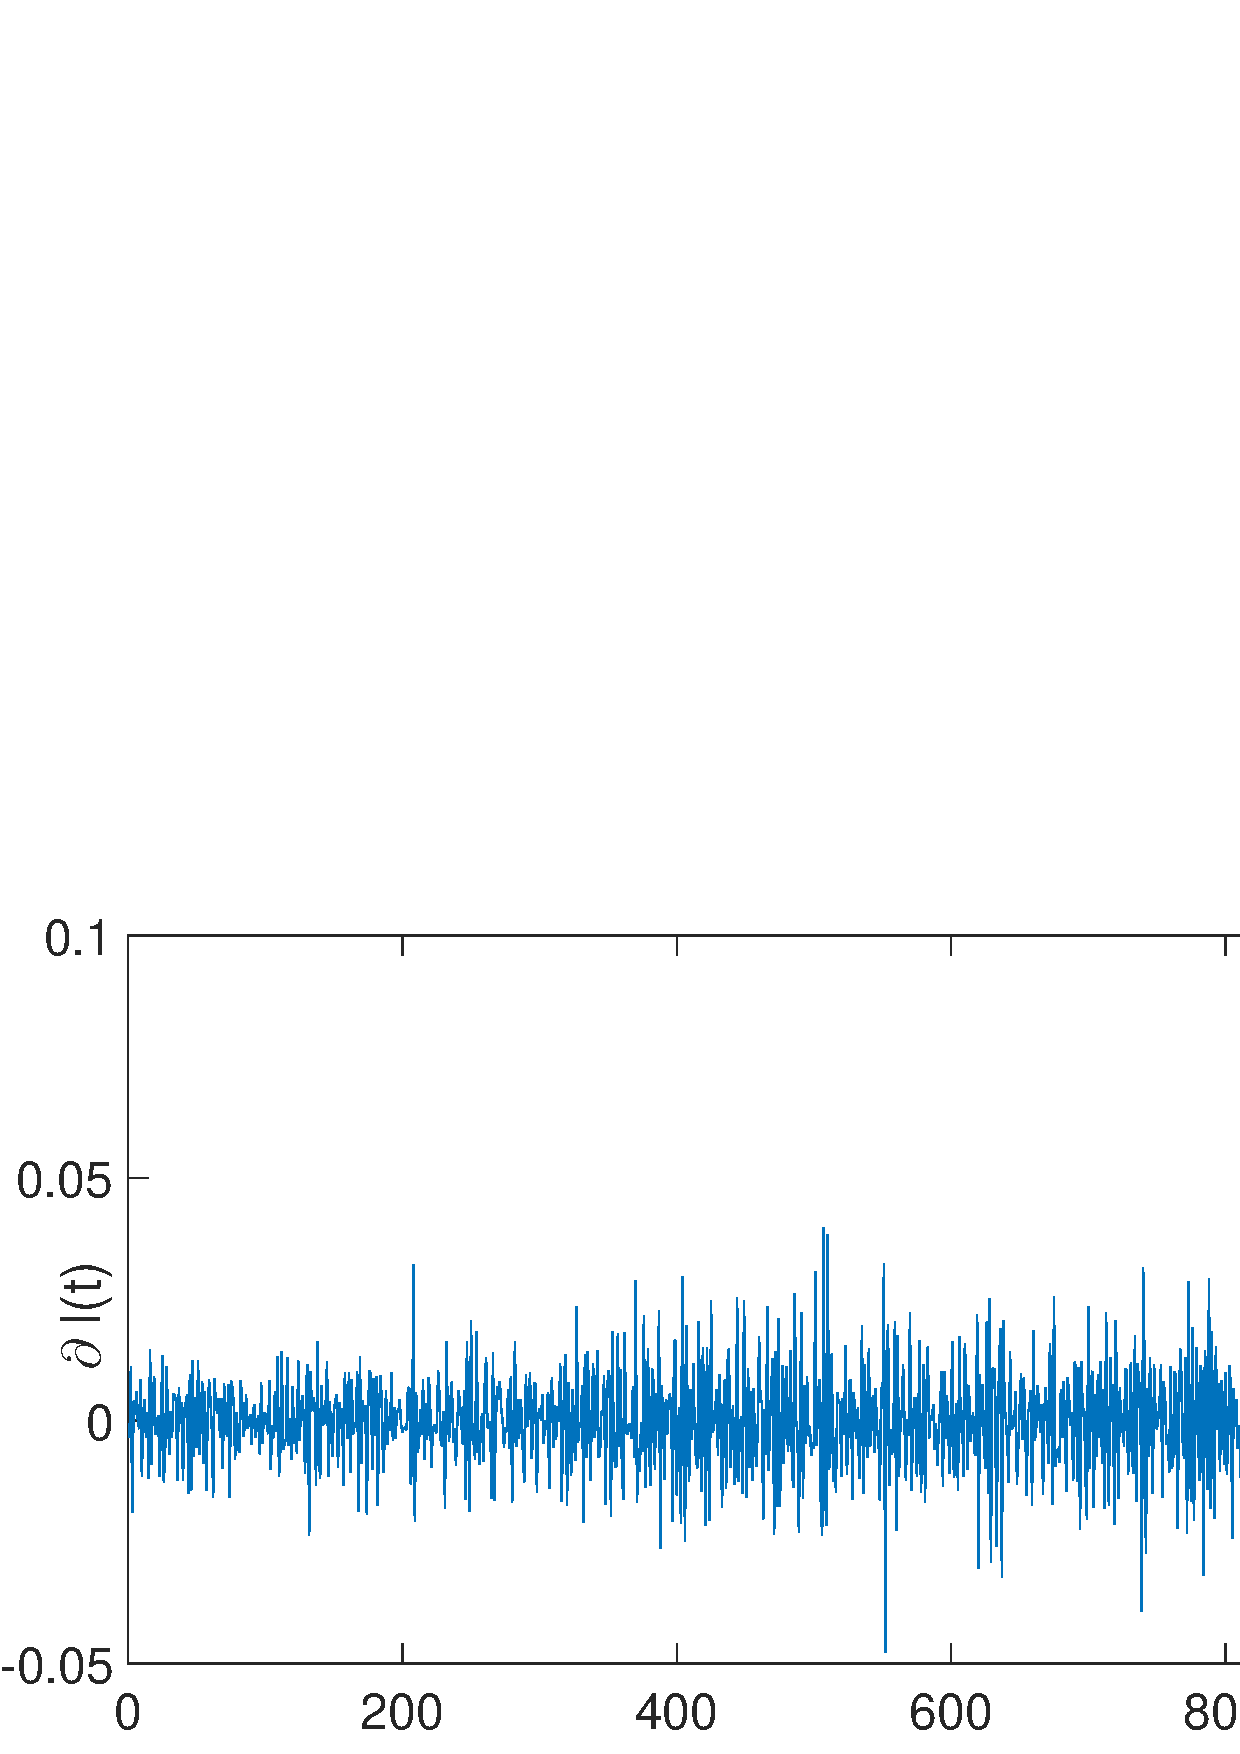
\includegraphics[width=12cm]{./pictures/Displacement/DISPLACEMENT_luma_detr}}
	\end{subfigure}
	\caption[Energia media della luma e suo detrending nel caso di uno spostamento della camera]
	{In questo esempio vediamo il comportamento dell'energia media della luma su una sequenza di 24 ore in cui avviene un evento di spostamento della camera.
		In (a) sono riportati alcuni frame estratti dalla sequenza. 
		Lo spostamento della camera avviene al frame $1000$ e, per il resto della sequenza, l'inquadratura rimane la stessa.
		In (b) vediamo il comportamento dell'indicatore $l(t)$, e in (c) quello del suo detrending.
		Vediamo come in (b) l'evento di spostamento della camera si traduca in un salto del valore di $l(t)$.
		In (c), invece, vediamo che l'evento si traduce in un picco (in questo caso positivo) nel valore del detrending nell'istante in cui inizia la sfocatura.}
	\label{fig:displacementDetrPLOT}
\end{figure}
%\clearpage
\noindent Possiamo vedere come, in generale, l'evento di tampering sia associato a un brusco salto o a un crollo \textit{istantaneo} del valore di uno o entrambi gli indicatori.
Vanno notate alcune cose:
\begin{itemize}
	\item L'evento di sfocatura non si traduce in un cambiamento nell'energia media della luma.
	Questo avviene perch\'e questo tipo di tampering abbatte le alte frequenze presenti nell'immagine, mantenendo comunque il valore medio della luma invariato.
	\item Facendo il detrending della sequenza abbiamo dei valori che oscillano attorno allo zero, un picco in corrispondenza dell'istante in cui avviene il tampering (Figure \ref{fig:energyDetrDefocus}, \ref{fig:energyDetrDisplacement}, \ref{fig:lumaDetrDisplacement}) e infine altri valori che oscillano attorno allo zero.
	Questo \`e dato dal fatto che il detrending considera le differenze tra dati consecutivi e, quindi, la differenza maggiore si ha proprio nell'istante in cui inizia l'evento di tampering, mentre solitamente le differenze tra misure consecutive sono minime. 
	Questo fa s\`i che monitorare il detrending delle sequenze degli indicatori permetta di identificare pi\`u facilmente gli eventi di tampering rispetto ad analizzare la sequenza originale.
	Il risvolto della medaglia \`e che i cambiamenti \textit{persistenti}, come quelli che stiamo considerando noi, diventano dei cambiamenti \textit{istantanei}.
	\item Considerando l'evento di sfocatura, possiamo notare (Figura \ref{fig:energyDefocus}) come, in seguito all'evento, oltre ad aver un crollo istantaneo del valore dell'energia del gradiente, abbiamo anche un abbassamento \textit{persistente} della sua varianza.
	Questo permette di utilizzare tecniche di monitoraggio sequenziale sull'energia del gradiente, con dei CDT sulla varianza, per identificare eventi di sfocatura.
\end{itemize}
In definitiva, \`e possibile identificare un evento di tampering andando a monitorare il detrending degli indicatori descritti da \eqref{eq:energyGradient} e \eqref{eq:energyLuma}, utilizzando semplicemente delle soglie in modo da individuare il picco causato dall'evento di tampering.
In particolare possiamo monitorare l'energia media del gradiente per individuare eventi di sfocatura, e l'energia media della luma per individuare eventi di spostamento della camera.
Inoltre, per rendere pi\`u robusta l'identificazione di sfocature, \`e possibile usare un test sequenziale sull'energia media del gradiente in grado di individuare dei cambiamenti nella varianza.
Dato il \textit{basso carico computazionale} richiesto da queste tecniche, \`e possibile integrarle su dispositivi embedded a basso consumo di energia.\\
Dobbiamo fare un'ultima considerazione sullo spostamento della camera.
Ci possono essere dei casi in cui l'evento \`e difficilmente individuabile monitorando la scena nella sua totalit\`a.
%\cleartoevenpage
\begin{figure}[tbp]
	\centering
	\begin{subfigure}[]
		{\label{fig:collage7} \includegraphics[width=12cm]{./pictures/buenosAiresCollageDisplacementBRUTTO}}
	\end{subfigure}
	\begin{subfigure}[]{\label{fig:lumaDisplacementBRUTTO} 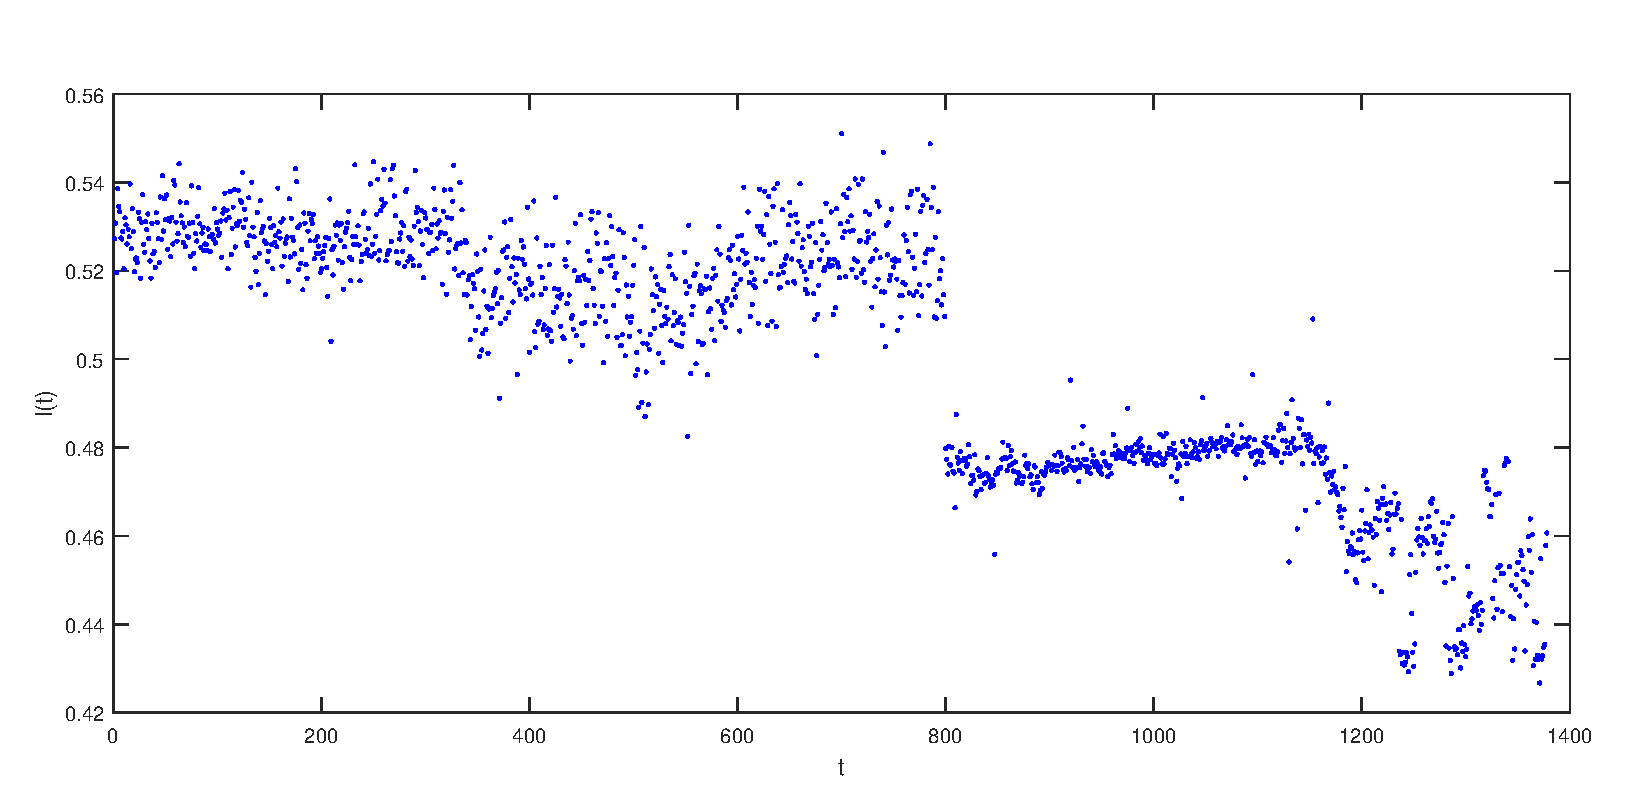
\includegraphics[width=12cm]{./pictures/DisplacementTOTALE/luma}}
	\end{subfigure}
	\begin{subfigure}[]
		{\label{fig:lumaDetrDisplacementBRUTTO} 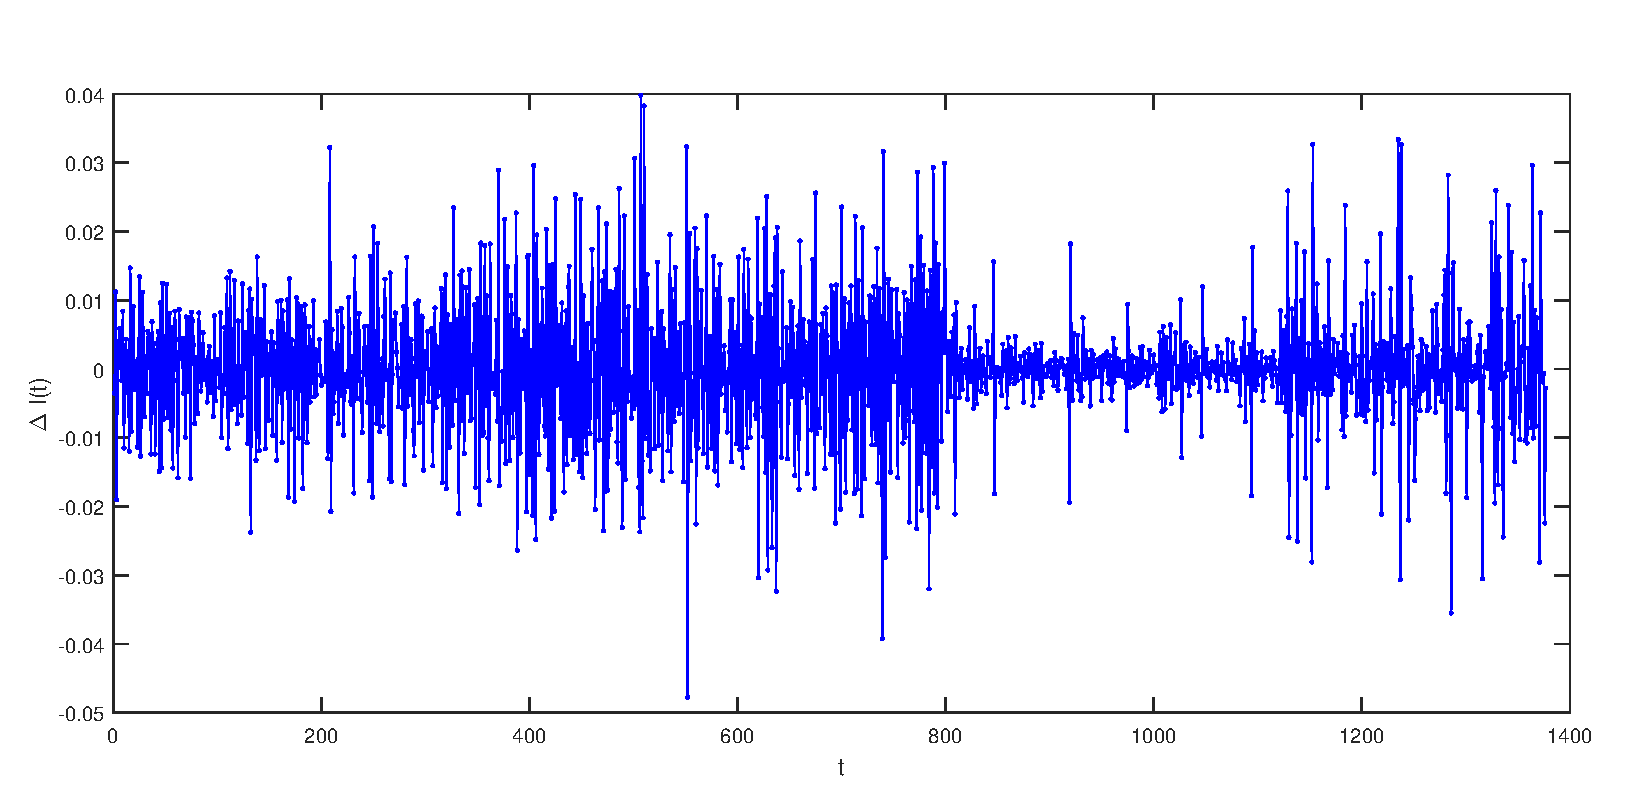
\includegraphics[width=12cm]{./pictures/DisplacementTOTALE/lumaDetr}}
	\end{subfigure}
	\caption[Esempio di sequenza dell'energia media della luma  e del suo detrending  con un displacement difficile da identificare]
	{In questo esempio vediamo il comportamento dell'energia media della luma su una sequenza di 24 ore in cui avviene un evento di spostamento della camera.
		In (a) sono riportati alcuni frame estratti dalla sequenza. 
		Lo spostamento della camera avviene al frame 
		$800$ e, per il resto della sequenza, l'inquadratura rimane la stessa.
		In (b) vediamo il comportamento dell'indicatore $l(t)$, e in (c) quello del suo detrending.
		Notiamo come, in (c), non abbiamo un picco ben distinguibili dagli altri valori nell'istante in cui avviene lo spostamento, come nella Figura \ref{fig:displacementDetrPLOT}.
		Questo problema capita perch\'e stiamo monitorando l'energia media della luma calcolata sulla \textit{totalit\`a} della scena.
		}
	\label{fig:displacementBRUTTO}
\end{figure}
%\clearpage
\begin{figure}[tb]
	\centering
	\subfigure[]{\label{fig:displacementORIGINALE1} 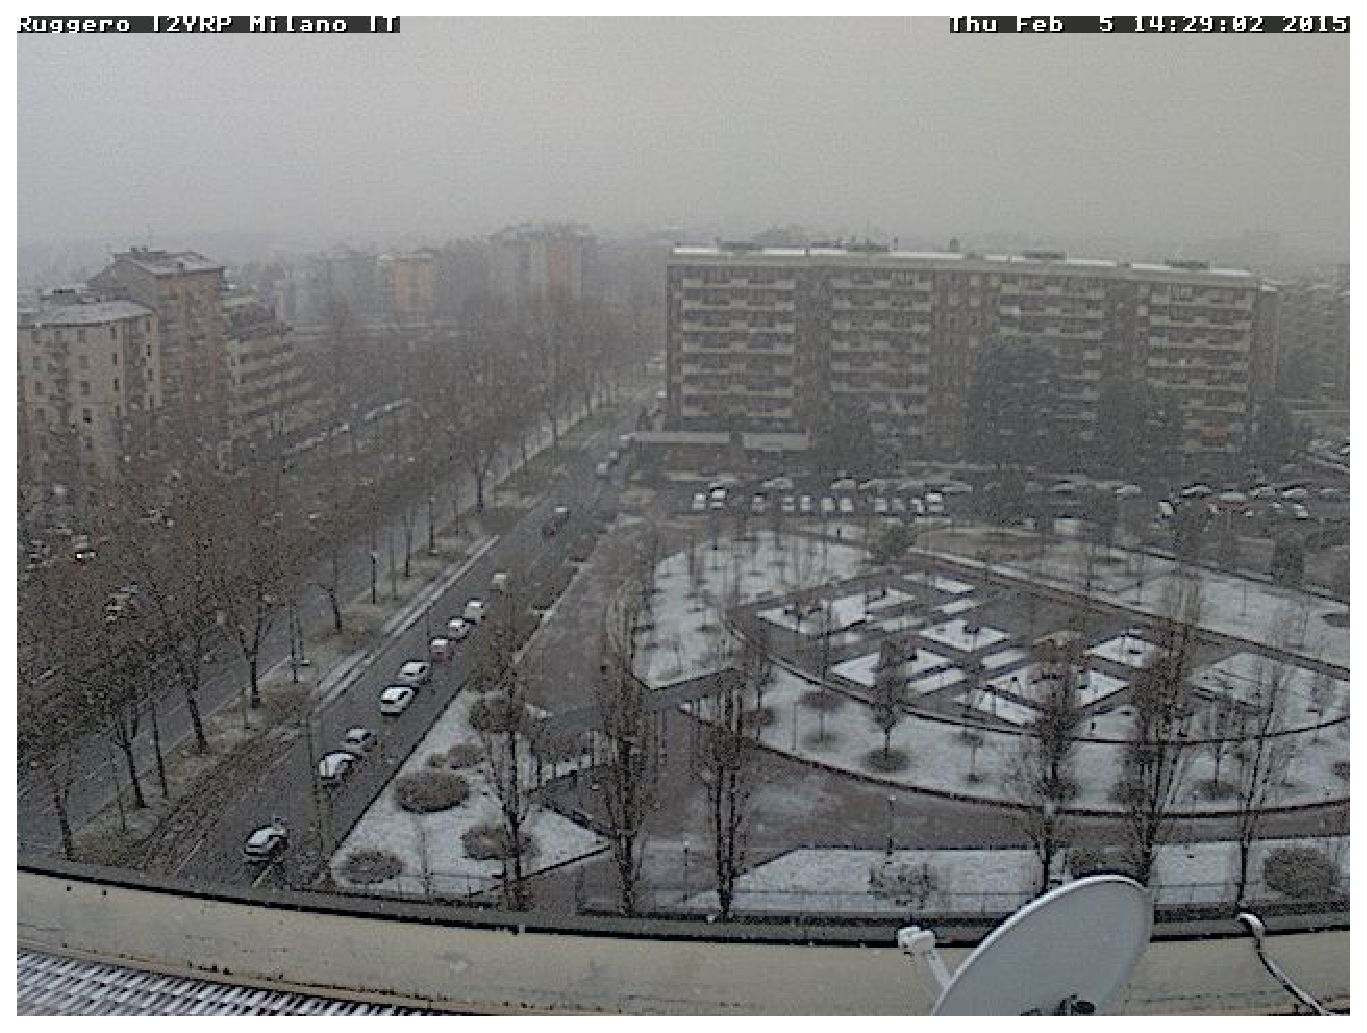
\includegraphics[width=6cm]{./pictures/testiORIGINALE}}
	\subfigure[]{\label{fig:displacementSPOSTATO1}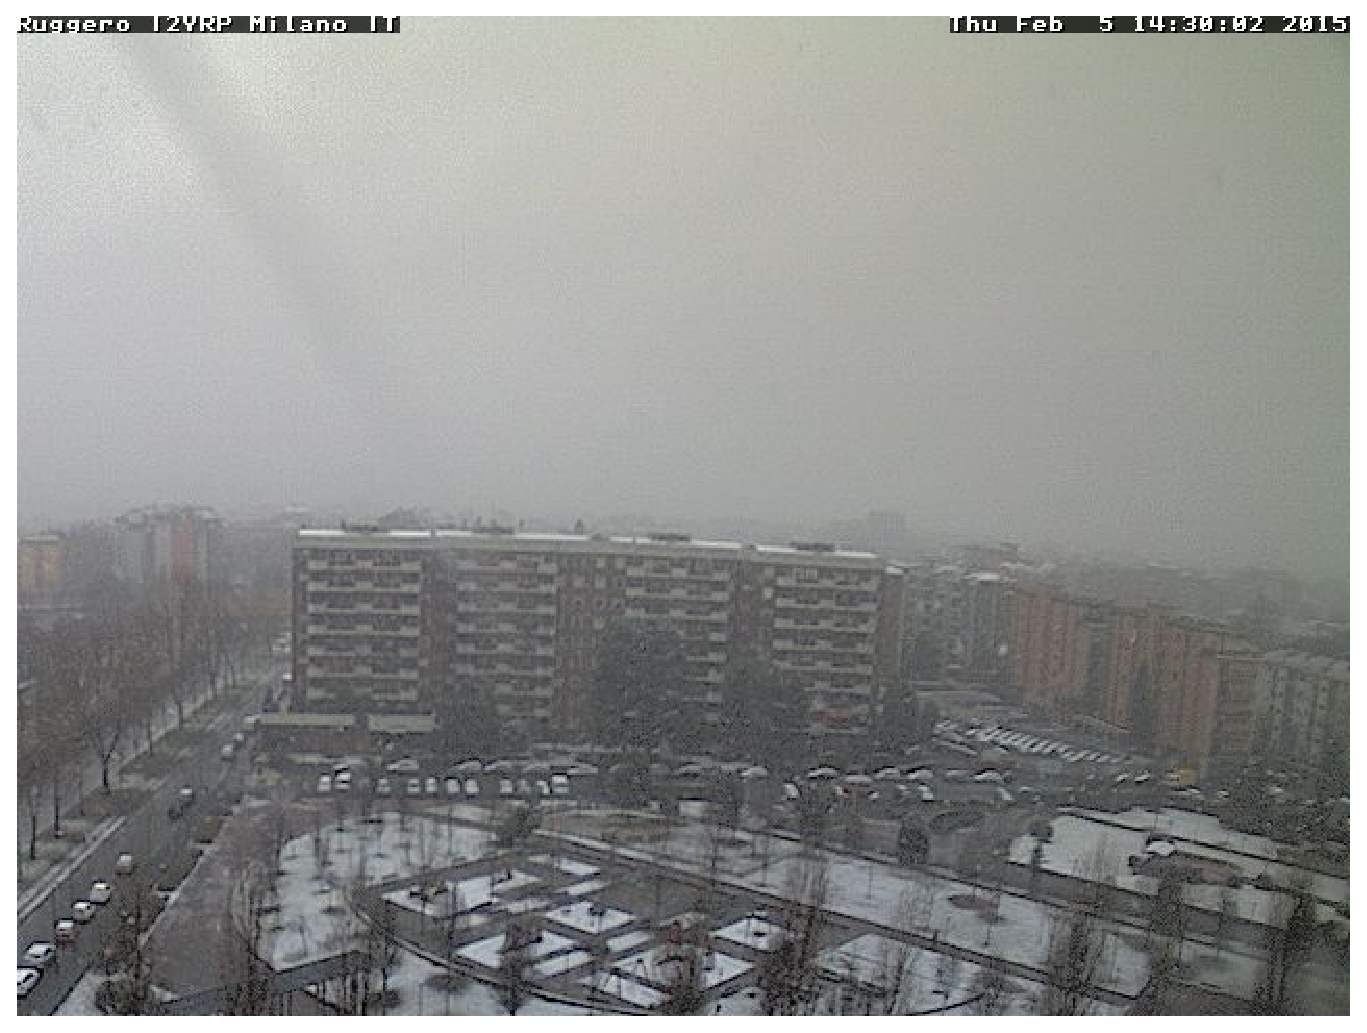
\includegraphics[width=6cm]{./pictures/testiDISPLACEMENT}}
	\caption{Esempio di spostamento della camera}
	\label{fig:testiDISPLACEMENT1}
\end{figure}
Un esempio \`e illustrato nella Figura \ref{fig:displacementBRUTTO}, dove vediamo un caso di spostamento della camera che avviene al frame $800$.
Questo evento, per\`o, non si traduce, nel segnale $\frac{\partial l}{\partial t}$, in un picco che si eleva rispetto agli altri, come nel caso della Figura \ref{fig:lumaDetrDisplacement}.
Questo problema capita perch\'e stiamo monitorando l'energia media della luma calcolata sulla \textit{totalit\`a} della scena.
Possiamo avere situazioni, come nel caso della Figura \ref{fig:displacementBRUTTO}, in cui lo spostamento della camera non determina un cambiamento sostanziale nella luminosit\`a media della scena.\\
Questo problema viene meno se consideriamo il contributo dell'energia della luma mediato non sulla totalit\`a della scena, bens\`i \textit{separatamente} su \textit{regioni} specifiche.
Infatti, se consideriamo un'area particolare della scena, come ad esempio quella occupata dal palazzo nella Figura \ref{fig:displacementORIGINALE1}, durante uno spostamento della camera la variazione della luma mediata solo sui pixel appartenenti a quella regione sar\`a pi\`u marcata rispetto a quella della luminosit\`a mediata su tutta l'immagine.
%Nella Figura  \ref{fig:testiDISPLACEMENT1}, tra il frame \ref{fig:displacementORIGINALE1} e il frame \ref{fig:displacementSPOSTATO1}, l'area occupata dal palazzo cambia il suo contenuto riprendendo un pezzo di cielo.
Questo ci ha suggerito di inserire una fase di \textit{segmentazione} in cui vengono estratte le regioni della scena che la camera deve inquadrare.
 \begin{figure}[tb]
 	\centering
 	\subfigure[]{\label{fig:testiSCENA} 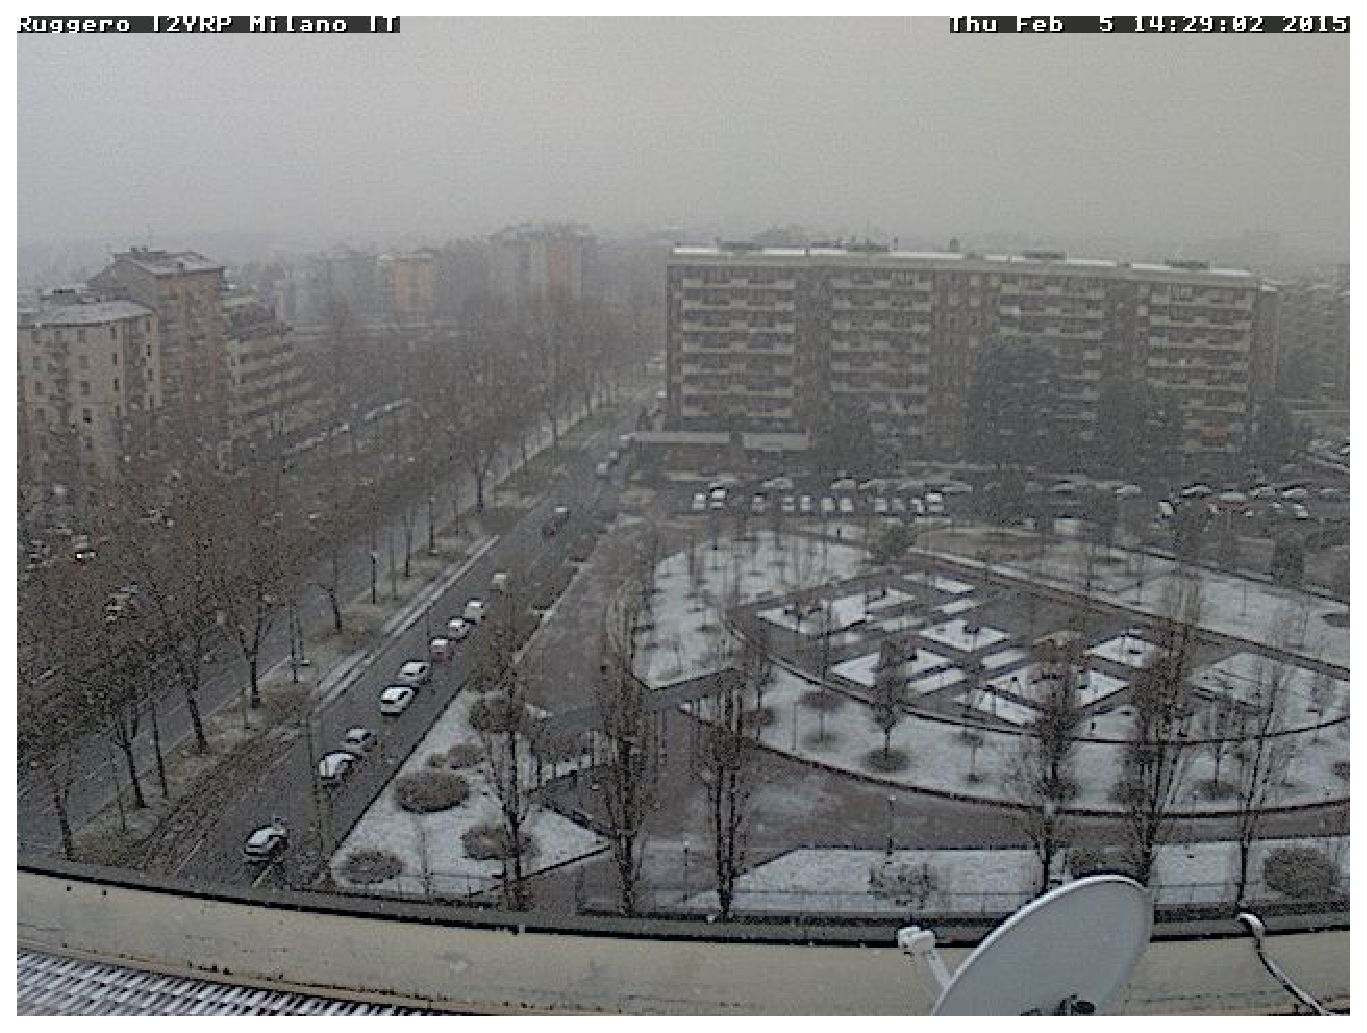
\includegraphics[width=6cm]{./pictures/testiORIGINALE}}
 	\subfigure[]{\label{fig:testiMAPPA}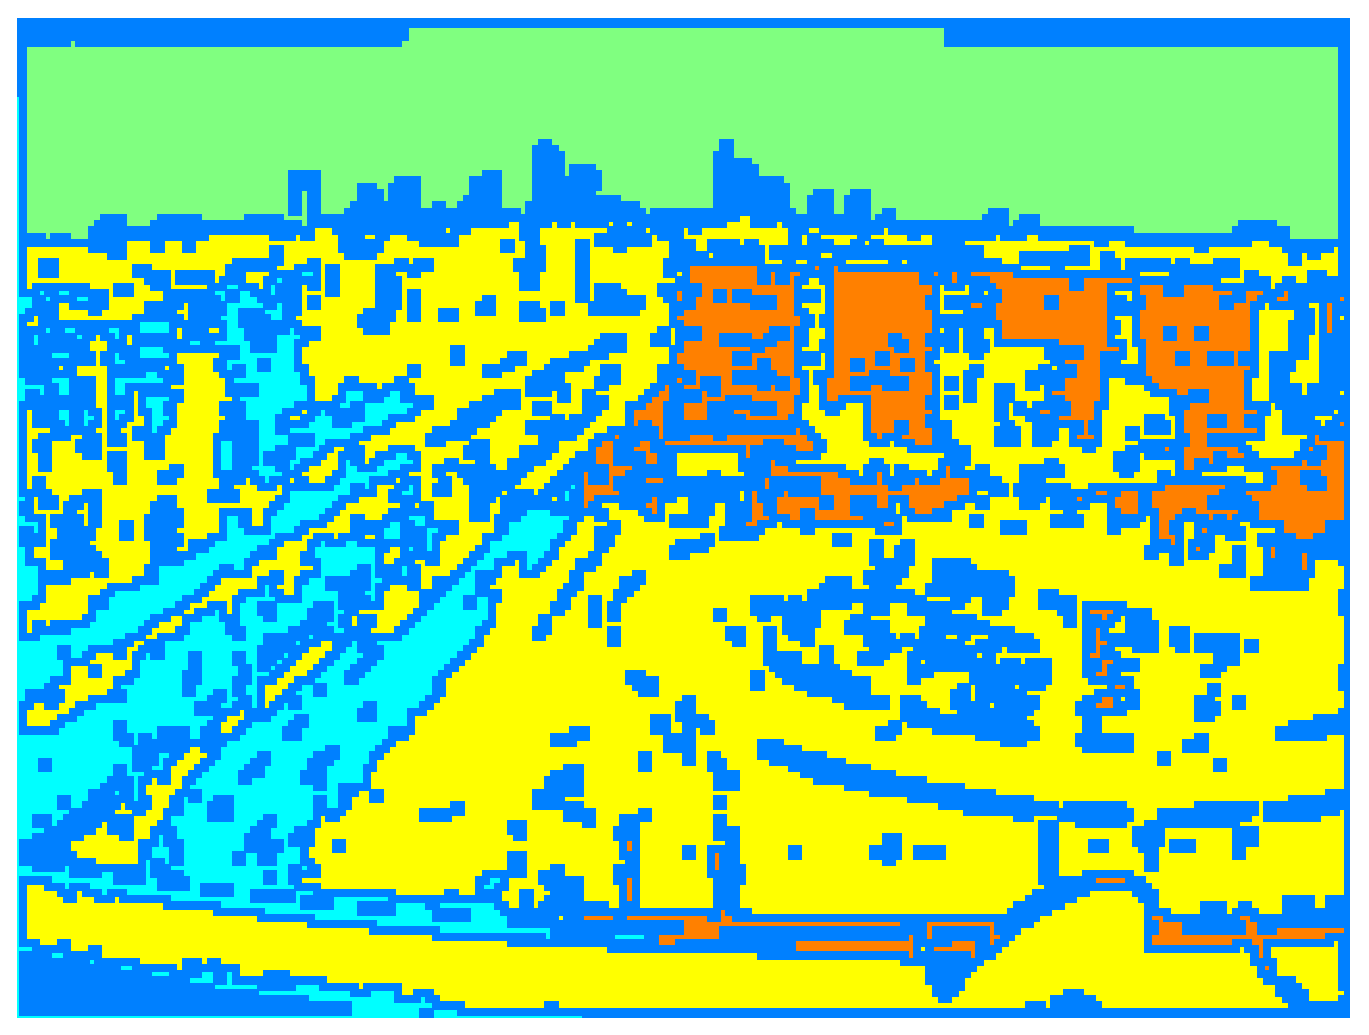
\includegraphics[width=6cm]{./pictures/map}}
 	\caption{Esempio di segmentazione della scena}
 	\label{fig:testiSEGMENTAZIONE}
 \end{figure}
Un esempio \`e illustrato nella Figura \ref{fig:testiSEGMENTAZIONE}. 
Nel Paragrafo \ref{segmentazione} vedremo in dettaglio come vengono estratte le regioni dalla scena.
\section{Algoritmo di identificazione di sfocature e di spostamenti della camera}
\label{monitoraggio}
In base alle considerazioni fatte nel Paragrafo \ref{indicatori} possiamo dividere l'algoritmo di tampering detection in due \textit{thread}:
il primo in grado di individuare la presenza di sfocature, il secondo lo spostamento della camera.
In particolare la presenza di sfocature pu\`o essere identificata monitorando l'energia media del gradiente, descritta in \eqref{eq:energyGradient}, mentre l'evento di spostamento della camera pu\`o essere identificato monitorando l'energia media della luma, descritta in \eqref{eq:energyLuma}.\\
In questo paragrafo illustriamo come sono state sviluppate le due tecniche.
\subsection{Identificazione delle sfocature}
\label{defocusDetection}
L'Algoritmo \ref{alg:DEFOCUS} mostra il funzionamento, ad alto livello, dell'algoritmo per identificare la presenza di sfocature nei frame.
%\IncMargin{0.1em}
%\vspace{-0.2cm}
\begin{algorithm}[t]
	% \SetAlgoNoLine
	\LinesNumbered
	\SetAlgoNlRelativeSize{0}
	\SetNlSty{small}{}{.}
	\textbf{Configurazione}:\\
	\lnl{DEF-Tr1} \For{$t=1,\dots,T_{o}$}
	{	\lnl{DEF-Tr2} Estraggo il frame $z_t$ \\
		\lnl{DEF-Tr3} Calcolo $g(t)$, $\frac{\partial g}{\partial t}(t)$ \\
	}
	\lnl{DEF-Tr4} Definisco le soglie $\Gamma_{min}^g$ e $\Gamma_{max}^g$\\
	\lnl{DEF-Tr5} Definisco i parametri per il CDT sulla varianza di $g(t)$\\
	\textbf{Fase operativa}:\\
	\lnl{DEF-Test1} \For{$t=T_{o},\dots,\infty$}{
		\lnl{DEF-Test2} Estraggo il frame $z_t$ \\
		\lnl{DEF-Test3} Calcolo $g(t)$, $\frac{\partial g}{\partial t}(t)$\\
		\lnl{DEF-Test4} \If{$\frac{\partial g}{\partial t}(t) < \Gamma_{min}^g \vee \frac{\partial g}{\partial t}(t) > \Gamma_{max}^g $}{
			\lnl{DEF-Test5} $z_t$ \`e un frame in cui \`e avvenuto una sfocatura\\
		}
		\lnl{DEF-Test8} \If{CDT identifica un cambiamento in $g(t)$}{
			\lnl{DEF-Test9} $z_t$ \`e un frame in cui \`e avvenuto uno spostamento della camera\\
		}
	}   
	\caption{Algoritmo di identificazione di sfocature}
	\label{alg:DEFOCUS}
\end{algorithm}
Dato che la sfocatura causa un crollo dell'energia media del gradiente e anche della sua varianza, \`e possibile lanciare due monitoraggi in grado di identificare ciascuno di questi cambiamenti, uno di tipo \textit{one-shot} e l'altro di tipo \textit{sequenziale}.\\
Il monitoraggio one-shot prevede un'analisi del detrending dell'energia media del gradiente, secondo \eqref{eq:energyGradient} e \eqref{eq:gradientDetr}, in modo da identificare il picco dovuto al cambiamento (si veda la Figura \ref{fig:defocusPLOT}).
L'identificazione viene fatta attraverso la definizione di due \textit{soglie}, calcolate facendo riferimento alle prime $T_{o}$ osservazioni, ritenute prive di tampering.
Tale sequenza prende il nome di \textit{training set}.
Le due soglie $\Gamma_{min}^g$ e $\Gamma_{max}^g$ vengono calcolate nel seguente modo:
\begin{equation}
\label{eq:soglieGradiente}
\begin{array}{lcl}
\Gamma_{min}^g & = & \widehat{\mu}_g -\gamma \widehat{\sigma}_g\\
\Gamma_{max}^g & = & \widehat{\mu}_g + \gamma \widehat{\sigma}_g
\end{array},
\end{equation}
dove $\widehat{\mu}_g$ indica il valore medio delle osservazioni del training set
\begin{equation}
	\widehat{\mu}_g = \frac{\sum_{\tau = 1}^{T_{o}} \frac{\partial g}{\partial t}(\tau)}{T_{o}}, \nonumber
\end{equation}
$\widehat{\sigma}_g$ indica la deviazione standard delle osservazioni del training set
\begin{equation}
\widehat{\sigma}_g  = \sqrt{\frac{1}{T_{o}-1}\sum_{\tau=1}^{T_{o}}\left(\frac{\partial g}{\partial t}(\tau) - \widehat{\mu}_g(\tau)\right)^2} \nonumber
\end{equation}
e $\gamma>1$ \`e un parametro moltiplicativo ottenuto sperimentalmente\footnote{Per maggiori dettagli si rimanda al Capitolo \ref{ProveSperimentali}}.\\
Le soglie definite in \eqref{eq:soglieGradiente} forniscono un limite superiore e uno inferiore ai valori di $\{\frac{\partial g}{\partial t}\}$ ammissibili.
Qualsiasi valore al di sotto di $\Gamma_{min}$ o al di sopra di $\Gamma_{max}$ viene considerato come un evento di sfocatura nel frame corrispondente.\\ 
Oltre all'analisi sul detrending \`e possibile fare un monitoraggio sequenziale sulla varianza di $\{g(t)\}$: infatti, come abbiamo visto nel Paragrafo \ref{comportamento}, la presenza di una sfocatura comporta una diminuzione della varianza di questa sequenza.
Il monitoraggio sequenziale viene fatto utilizzando un CDT basato su ICI-rule\footnote{Lo schema di funzionamento del CDT basato su ICI-rule \`e spiegato nel Paragrafo \ref{cdt}.} sulla varianza di $\{g(t)\}$, usando il training set per configurare i suoi parametri.


\subsection{Identificazione degli spostamenti della camera}
\label{monitoraggioDISPL}
L'Algoritmo \ref{alg:DISPL} mostra il funzionamento, ad alto livello, dell'algoritmo per identificare un evento di spostamento della camera.\\
\begin{algorithm}[t]
	% \SetAlgoNoLine
	\LinesNumbered
	\SetAlgoNlRelativeSize{0}
	\SetNlSty{small}{}{.}
	\textbf{Configurazione}:\\
	\lnl{DISPL-Tr1} Estraggo le regioni $\{R_k\}, k=1,\dots,K$  \\
	\lnl{DISPL-Tr2} \For{$t=1,\dots,T_{o}$}
	{	\lnl{DISPL-Tr3} Estraggo il frame $z_t$ \\
		\lnl{DISPL-Tr4} \For{$k=1,\dots,K$}{
			\lnl{DISPL-Tr5} Calcolo $l^k(t)$, $\frac{\partial l^k}{\partial t}(t)$ per la regione $R_k$\\
		}
	}
	\lnl{DISPL-Tr6} \For{$k=1,\dots,K$}{
		\lnl{DISPL-Tr7} Definisco le soglie $\Gamma_{min}^k$ e $\Gamma_{max}^k$\\
	}
	\textbf{Fase operativa}:\\
	\lnl{DISPL-Test1} \For{$t=T_{o},\dots,\infty$}{
		\lnl{DISPL-Test2} Estraggo il frame $z_t$ \\
		\lnl{DISPL-Test3} $n = 0$ \\
		\lnl{DISPL-Test4} \For{$k=1,\dots,K$}{
			\lnl{DISPL-Test5} Calcolo $l^k(t)$, $\frac{\partial l^k}{\partial t}(t)$ per la regione $R_k$\\
			\lnl{DISPL-Test6} \If{$\frac{\partial l^k}{\partial t}(t) < \Gamma_{min}^k \vee \frac{\partial l^k}{\partial t}(t) > \Gamma_{max}^k $}{
				\lnl{DISPL-Test7} $n=n+1$\\
			}
		}
		\lnl{DISPL-Test8} \If{$n\geq K-1$}{
			\lnl{DISPL-Test9} $z_t$ \`e un frame in cui \`e avvenuto uno spostamento della camera\\
		}
	}   
	\caption{Algoritmo di identificazione di spostamenti della camera}
	\label{alg:DISPL}
\end{algorithm}
Una prima fase dell'algoritmo consiste nella \textit{segmentazione} della scena inquadrata dalla camera in un insieme di regioni $\{R_k\}, k=1,\dots,K$.
Il metodo con cui vengono estratte queste regioni verr\`a analizzato in dettaglio nel paragrafo \ref{segmentazione}. \\
L'analisi che viene fatta \`e simile a quella vista nel monitoraggio del detrending dell'energia del gradiente:
in questo caso l'analisi \`e fatta in maniera indipendente per ciascuna regione $R_k$, calcolando l'energia della luma \textit{mediata per i pixel appartenenti alla regione}:
\begin{equation}
	\label{eq:lumaRegions}
	\begin{array}{ccc}
	l^k(t)&  = & \mathcal{L}^k[z_t] = \frac{\sum_{\mathcal{X}} z_t(x) }{|{R_k}|}\\
	\frac{\partial l^k}{\partial t}(t) & =& l^k(t)-l^k(t-1) 
	\end{array},
\end{equation}
dove abbiamo indicato con $|{R_k}|$ il numero totale dei pixel appartenenti alla regione $R_k$.\\
L'identificazione viene fatta attraverso la definizione di due \textit{soglie}, calcolate facendo riferimento alle prime $T_{o}$ osservazioni, ritenute prive di tampering.
Le due soglie $\Gamma_{min}^k$ e $\Gamma_{max}^k$ vengono calcolate per ciascuna regione nel seguente modo:
\begin{equation}
\label{eq:soglieLuma}
\begin{array}{rcl}
\Gamma_{min}^k & = & \widehat{\mu}_l^k -\gamma \widehat{\sigma}_l^k\\
\Gamma_{max}^k & = & \widehat{\mu}_l^k + \gamma \widehat{\sigma}_l^k
\end{array},
\end{equation}
dove $\widehat{\mu}_l^k$ indica il valore medio delle osservazioni del training set
\begin{equation}
\widehat{\mu}_l^k = \frac{\sum_{\tau = 1}^{T_{o}} \frac{\partial l^k}{\partial t}(\tau)}{T_{o}}, \nonumber
\end{equation}
$\widehat{\sigma}_l^k$ indica la deviazione standard delle osservazioni del training set
\begin{equation}
\widehat{\sigma}_l^k  = \sqrt{\frac{1}{T_{o}-1}\sum_{\tau=1}^{T_{o}}\left(\frac{\partial l^k}{\partial t}(\tau) - \widehat{\mu}_l^k(\tau)\right)^2} \nonumber
\end{equation}
e $\gamma>1$ \`e un parametro moltiplicativo ottenuto sperimentalmente.\\
Le soglie definite nella Formula \eqref{eq:soglieLuma} forniscono un limite superiore e uno inferiore ai valori di $\{\frac{\partial l^k}{\partial t}\}$ ammissibili.\\
Dato che l'evento di spostamento della camera viene inteso come un cambiamento globale dell'immagine, ci aspettiamo che tale cambiamento sia percepibile in tutte le regioni contemporaneamente. 
Nella pratica, per\`o, pu\`o capitare che l'energia media della luma all'interno di una specifica regione non cambi, anche in caso di spostamento della camera.
Se consideriamo, ad  esempio, l'evento di spostamento nella Figura \ref{fig:displacementBRUTTO} e la segmentazione della scena in Figura \ref{fig:testiMAPPA}, infatti, possiamo notare come la luma nella regione del cielo non subisca cambiamenti sostanziali dato che, anche in seguito all'evento di tampering, questa regione riprende sempre una porzione di cielo.\\
In generale, quindi, possiamo considerare un monitoraggio indipendente di ogni sequenza $\{\Delta l_t^k\}$ per $k=1,\dots,K$.
Se, all'istante $T^*$, abbiamo che, per $K-1$ regioni sulle $K$ totali, il valore di $\Delta l_{T^*}^k$ \`e maggiore di $\Gamma_{max}^k$ o minore di $\Gamma_{min}^k$, allora possiamo considerare avvenuto un evento di sfocatura nel frame $z_{T^*}$. \\ 
Dato che l'evento di spostamento della camera, in genere, non comporta un cambiamento persistente nella varianza dell'energia media della luma, non ha senso aggiungere un monitoraggio sequenziale come abbiamo fatto nell'Algoritmo \ref{alg:DEFOCUS}.
\section{Algoritmo di segmentazione}
\label{segmentazione}
In molte applicazioni di visione artificiale \`e spesso necessario estrarre, da un'immagine o un video, una o pi\`u regioni specifiche. Quando si vanno a trattare dei video, i tipi di segmentazione che possono essere applicati sono solitamente due:
\begin{itemize}      
	\item una segmentazione di tipo \textit{spaziale}, in cui vengono estratti dei pixel specifici per ogni frame costituente il video;
	\item una segmentazione di tipo \textit{temporale}, in cui vengono estratti dei frame significativi (\textit{key-frames}).
\end{itemize}
Segmentazioni di tipo spaziale permettono, ad esempio, di seguire il movimento di uno specifico oggetto all'interno della scena ripresa \cite{kim2003efficient,kottke1994motion}, oppure di identificare un particolare evento all'interno di una scena \cite{ke2007event}.
Alcuni standard video, come ad esempio l'MPEG-4, utilizzano una codifica \textit{object-based} in cui viene utilizzata una segmentazione spaziale dei frame \cite{deng2001unsupervised}. 
Segmentazioni di tipo temporale, invece, permettono di dividere un filmato in \textit{sottosequenze} oppure di creare una sintesi del video con dei frame significativi. In quest'ultimo caso si parla di \textit{key-frames extraction} o di \textit{video summarization} \cite{gong2000video,jiang2009hierarchical,sentinelli2014live,wolf1996key}. Quando si vanno a trattare immagini la segmentazione \`e di tipo spaziale.\\
Considerando la segmentazione di tipo spaziale, una soluzione molto diretta consiste nell'utilizzare dei descrittori per ciascun pixel e applicare delle tecniche di \textit{clustering}, ovvero delle metodologie atte a partizionare un insieme di dati \cite{han2006data}, sugli stessi. \\
Nel Paragrafo \ref{comportamento} abbiamo introdotto il fatto di utilizzare una segmentazione in regioni della scena ripresa dalla camera, in modo da rendere pi\`u efficiente l'identificazione di spostamenti della camera.
Vediamo ora il modo in cui questa segmentazione viene fatta.\\
Durante la fase di estrazione delle regioni acquisiamo un certo numero di frame in cui non avviene nessun evento di tampering.
Da questi frame estraiamo un vettore descrittore (\textit{feature vector}) per ciascun pixel della scena inquadrata.
Passiamo, quindi, da una matrice di dimensioni $H\times W \times T_{c}$, dove $H$ e $W$ sono le dimensioni in pixel dell'immagine acquisita dalla camera e $T_{c}$ \`e il numero di frame usato per la creazione della segmentazione, a una matrice di dimensioni $H\times W \times P$, dove $P$ \`e il numero di descrittori calcolati per fare la segmentazione.\\
Una volta ottenuta la matrice, vengono raggruppati i pixel aventi feature vector simili tramite tecniche di \textit{clustering}.\\
La fase di segmentazione della scena in regioni avviene durante la configurazione del sistema, separatamente rispetto alla fase di identificazione degli eventi di tampering.
La segmentazione, quindi, non comporta ulteriore costo computazionale all'algoritmo, in cui viene considerata semplicemente come una variabile d'ingresso.
Inoltre, la segmentazione pu\`o essere eseguita \textit{offline} su un dispositivo esterno.
\begin{figure}
	\centering
	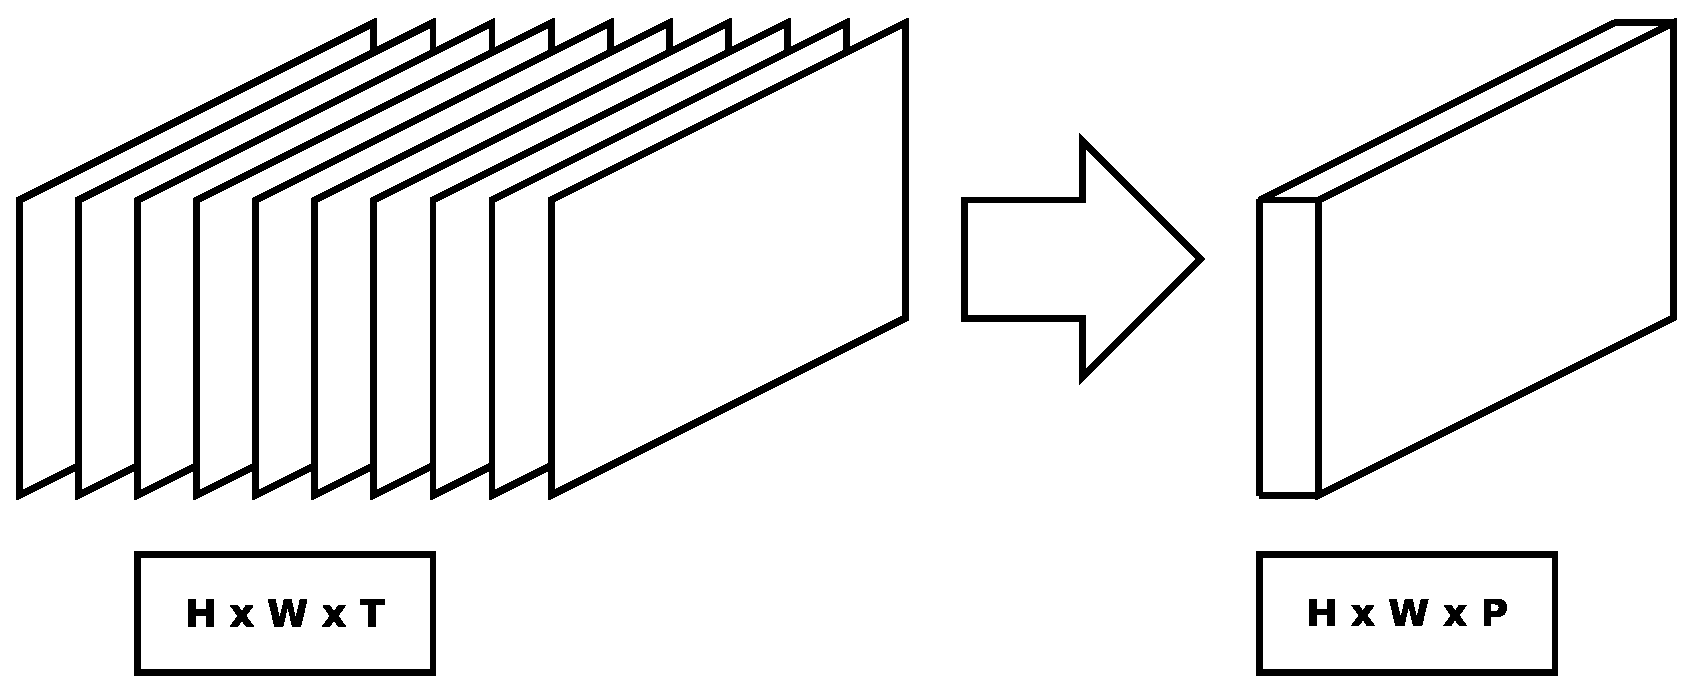
\includegraphics[width=0.7\linewidth]{diagrammi/FeatureVector}
	\caption{Passaggio dallo spazio dei frame allo spazio dei feature vector}
	\label{fig:FeatureVector}
\end{figure}

\subsection{Calcolo dei descrittori utilizzati per la segmentazione}
\label{descrittori}
Consideriamo la sequenza $\{z_t\}$ di frame acquisiti dalla camera, con $t=1,\dots,T_{c}$.
Per ciascun pixel $x\in\mathcal{X}$ calcoliamo un vettore $\textbf{d}(x)$ di $5$ elementi
\begin{equation}
	\label{eq:featureVector}
	\textbf{d}(x)=\left[r(x);c(x);\mu_{\nabla}(x);\sigma_{\nabla}(x);\bar{z}(x)\right], \textbf{d}(x) \in \mathbb{R}^5
\end{equation}
dove:
\begin{itemize}
	\item $r(x)$ rappresenta il numero di riga del pixel $x$.
	\item $c(x)$ rappresenta il numero di colonna del pixel $x$.
	\item $\mu_{\nabla}(x)$ rappresenta il valore del gradiente nel pixel $x$ mediato nel tempo:
	\begin{equation}
	\label{eq:segmentazioneGrad}
		\mu_{\nabla}(x) = \frac{\sum_{t=1}^{T_c}(\|\nabla z_t\|_2^2 \circledast f)(x)}{T_c},
	\end{equation}
	dove abbiamo indicato con $\|\nabla z_t\|_2^2$ la norma del gradiente per l'immagine $z_t$, definita in \eqref{eq:normaGradiente}, e con $f$ il filtro gaussiano discreto derivato dal campionamento di \eqref{eq:gaussian}.
	\item $\sigma_{\nabla}(x)$ rappresenta la deviazione standard nel tempo del gradiente nel pixel $x$:
	\begin{equation}
		\label{eq:segmentazioneVar}
		\sigma_{\nabla}(x)=\sqrt{\frac{1}{T_c - 1}\sum_{t=1}^{T_c}\left(\left(\|\nabla z_t\|_2^2 \circledast f\right)(x)-\mu_{\nabla}(x)\right)^2}.
	\end{equation}
	\item $\bar{z}(x)$ rappresenta il valore della luma del pixel $x$ mediato nel tempo:
	\begin{equation}
	\label{eq:segmentazioneLuma}
	\bar{z}(x)=\frac{\sum_{t=1}^{T_c}( z_t \circledast f)(x)}{T_c}.
	\end{equation}
\end{itemize}
Come possiamo vedere in \eqref{eq:segmentazioneGrad}, \eqref{eq:segmentazioneVar} e \eqref{eq:segmentazioneLuma}, nel calcolo degli indicatori viene fatta una convoluzione con un filtro gaussiano.
Questo \`e equivalente a mediare il contributo di $\|\nabla z_t\|_2^2$ e di $z_t$ in un \textit{intorno spaziale}.\\
Nella Figura \ref{fig:FVexample} possiamo vedere un esempio di come si comportano questi indicatori su una specifica scena (Figura \ref{fig:FVframe}).
Il loro utilizzo permette di avere un'informazione completa sul comportamento dei pixel durante la ripresa della scena e il loro rapporto con i pixel appartenenti al suo intorno, definito dal filtro gaussiano $f$.\\
In particolare, l'indicatore $\mu_{\nabla}(x)$ mette in relazione il valore di luma del pixel $x$  con quelli nel suo intorno, definito dal filtro $f$. 
Valori alti di $\mu_{\nabla}(x)$ corrispondono a zone della scena con molti dettagli (\textit{textured}), mentre valori bassi corrispondo a zone della scena poco dettagliate (\textit{flat}).
\begin{figure}[tb]
	\centering
	\begin{subfigure}[]
		{\label{fig:FVframe} 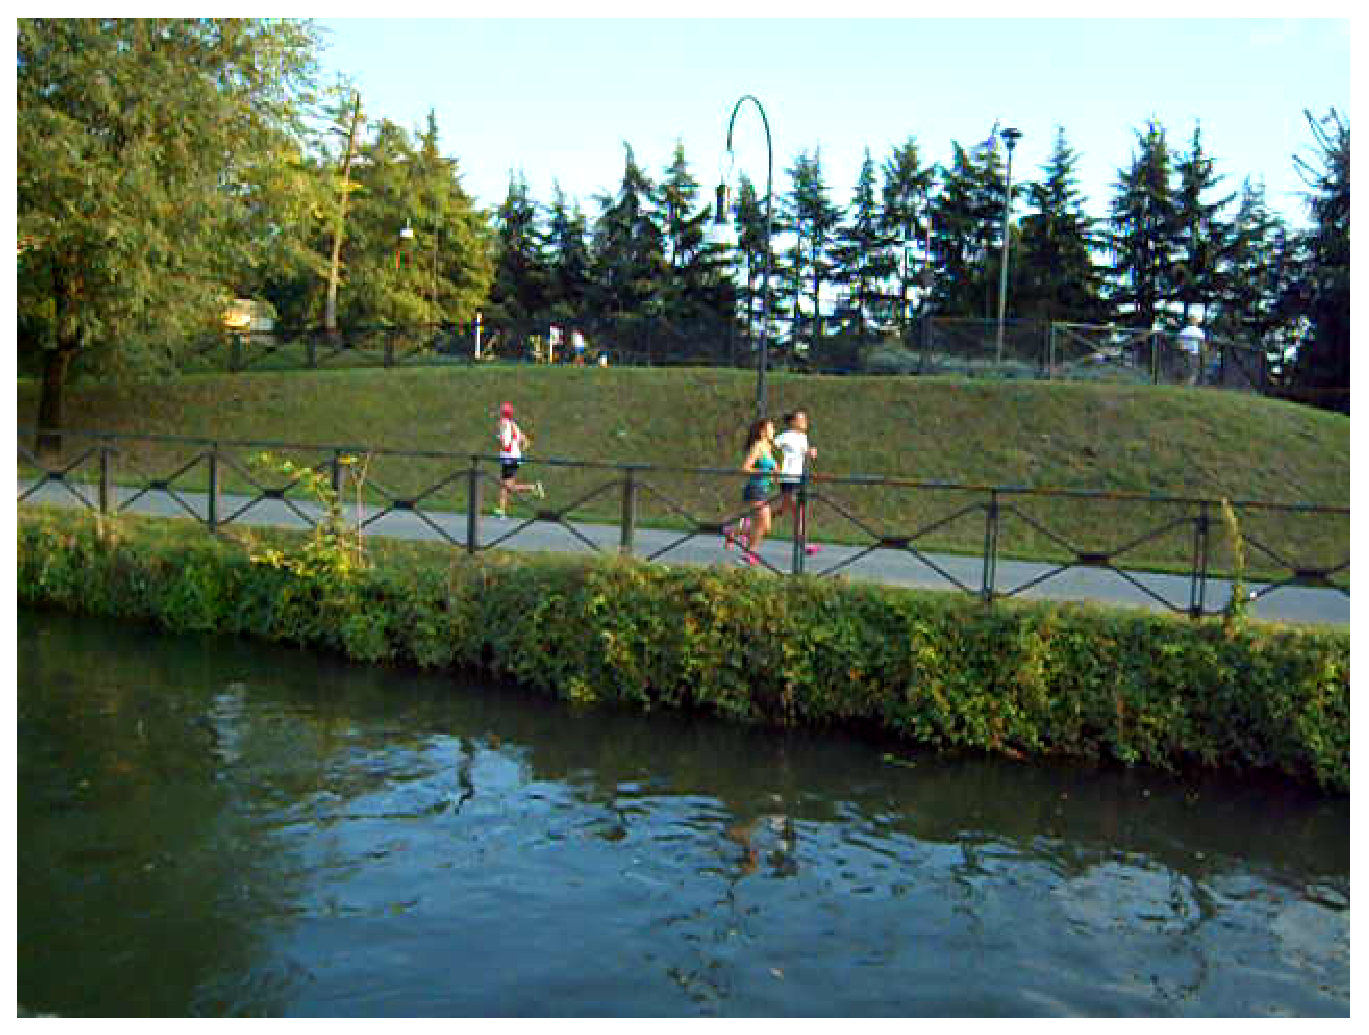
\includegraphics[width=6cm]{./pictures/FeatureVector/frame}}
	\end{subfigure}
	\begin{subfigure}[]
		{\label{fig:FVgrad} 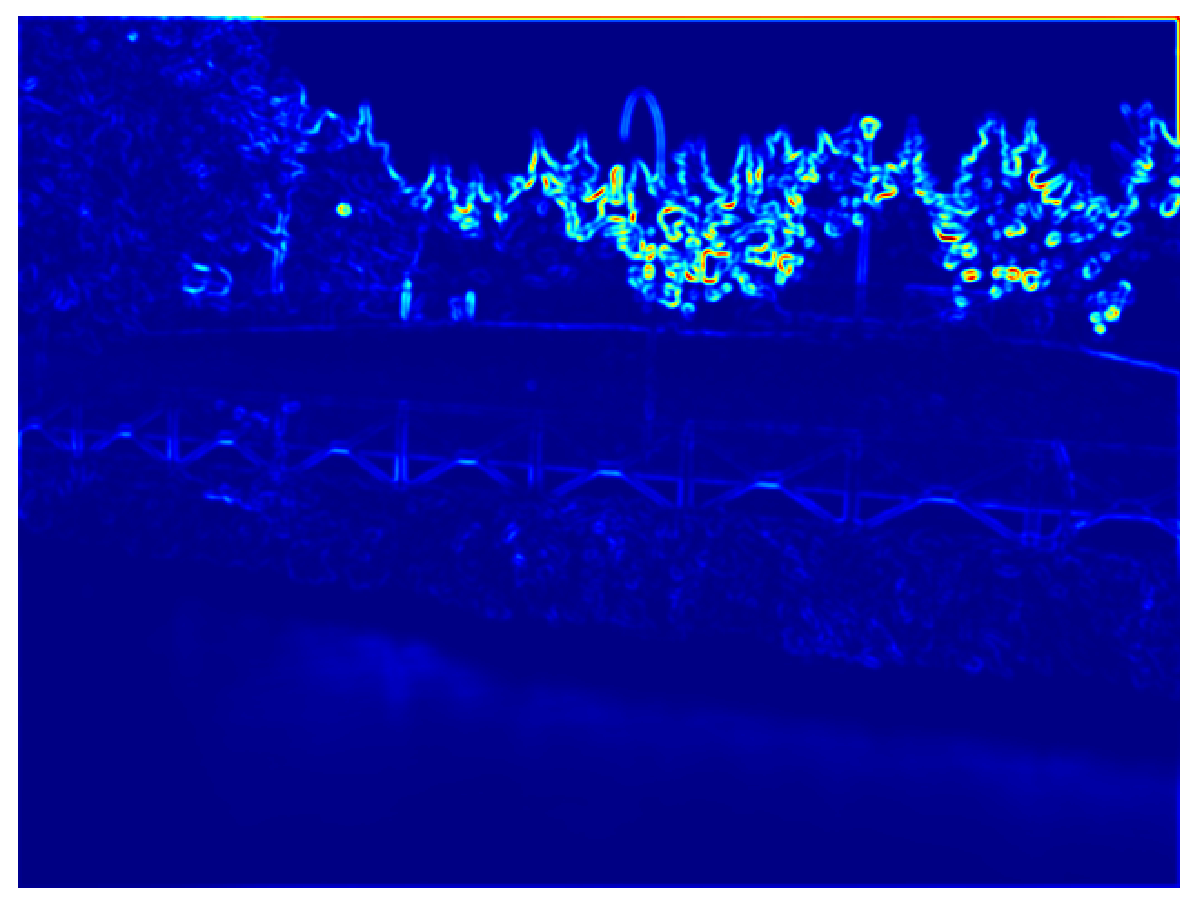
\includegraphics[width=6cm]{./pictures/FeatureVector/spatialGrad}}
	\end{subfigure}
	\begin{subfigure}[]
		{\label{fig:FVstd} 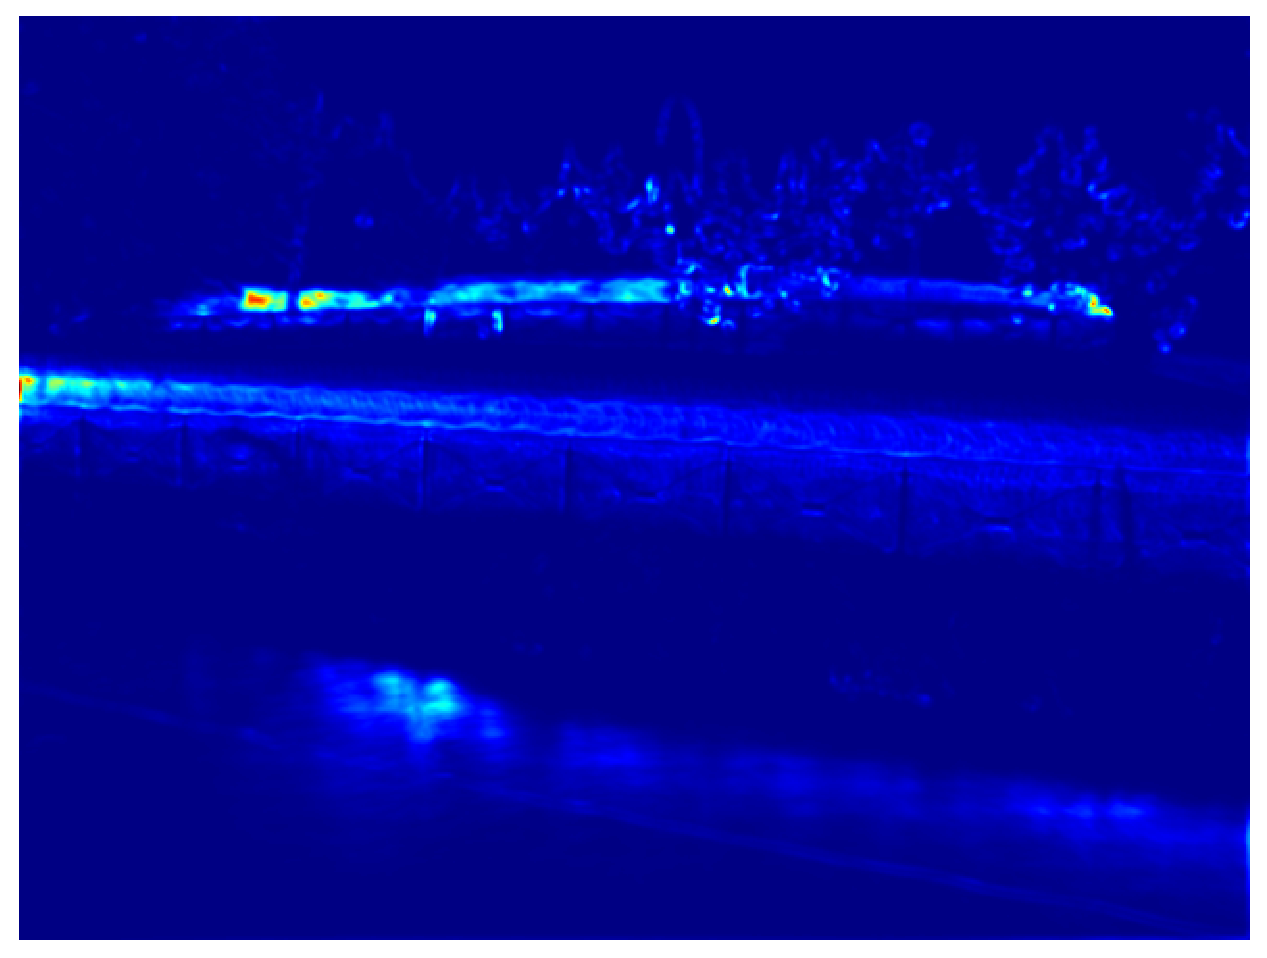
\includegraphics[width=6cm]{./pictures/FeatureVector/stdGrad}}
	\end{subfigure}
	\begin{subfigure}[]
		{\label{fig:FVluma} 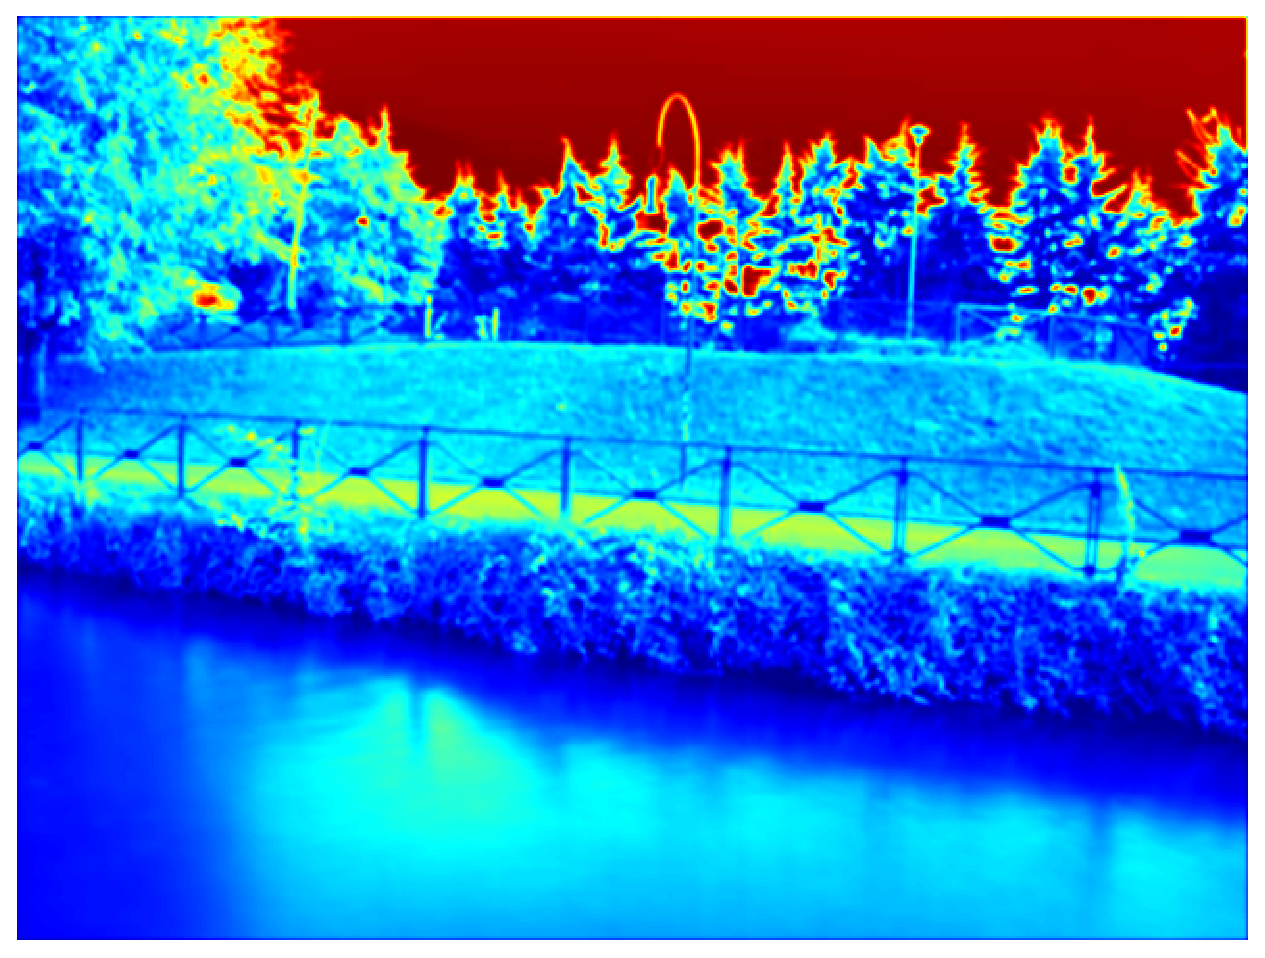
\includegraphics[width=6cm]{./pictures/FeatureVector/meanLuma}}
	\end{subfigure}
	\caption[Descrittori per la segmentazione della scena]
	{Esempio grafico di come si comportano i descrittori utilizzati per la segmentazione di una specifica scena. 
	La scena di esempio \`e rappresentata in (a).
	In (b), dove sono illustrati i valori di $\mu_{\nabla}(x)$ per ciascun pixel, possiamo vedere come i valori pi\`u alti siamo in prossimit\`a delle zone pi\`u dettagliate, come per esempio il contorno tra le foglie e il cielo.
	In (c), invece, vediamo i valori di $\sigma_{\nabla}(x)$ per ciascun pixel.
	Possiamo notare come i valori pi\`u alti del descrittore siano in prossimit\`a delle zone a maggior dinamicit\`a, come ad esempio la zona dove passano le persone.
	In (d), infine, mostriamo i valori di $\bar{z}(x)$ per ciascun pixel.}
	\label{fig:FVexample}
\end{figure}
Ad esempio, nella Figura \ref{fig:FVgrad} possiamo vedere come i valori pi\`u alti di $\mu_{\nabla}(x)$ corrispondano alle zone dove le variazioni di luma sono pi\`u elevate (ad esempio nelle aree di contorno tra le foglie degli alberi e il cielo).\\
L'indicatore $\sigma_{\nabla}(x)$, invece, ci fornisce un'informazione riguardo all'evoluzione di ciascun pixel nel tempo.
Valori alti di $\sigma_{\nabla}(x)$ corrisponderanno a pixel appartenenti a zone \textit{dinamiche} della scena, mentre valori bassi dell'indicatore corrisponderanno a pixel appartenenti a zone \textit{statiche}.
Nell'esempio in Figura \ref{fig:FVstd} possiamo vedere come i valori pi\`u alti dell'indicatore corrispondano alle zone dove passano i pedoni e i ciclisti.\\
L'indicatore $\bar{z}$ (Figura \ref{fig:FVluma}) ci fornisce un'indicazione su come \`e distribuita mediamente, su un intorno spaziale, la luminosit\`a nella scena.\\
L'utilizzo delle coordinate spaziali, infine, permette di avere un'informazione sulla posizione del pixel all'interno della scena.
\subsection{Partizionamento dei feature vector per l'estrazione delle regioni}
Una volta calcolati i feature vector di tutti i pixel, possiamo raggrupparli tra loro usando un algoritmo di \textit{clustering}.
In realt\`a, per alleggerire il peso computazionale nella fase di segmentazione, possiamo fare un \textit{sottocampionamento} dei feature vector totali.
Come abbiamo visto nel Paragrafo \ref{descrittori}, infatti, ciascun feature vector \`e associato non al singolo pixel, ma a un intorno del pixel definito dal filtro gaussiano $f$.
Possiamo, quindi, dividere la scena totale in \textit{blocchi}, le cui dimensioni sono paragonabili a quelle del filtro $f$, e prendere il feature vector del pixel centrale di ciascun blocco.\\ 
Per partizionare i feature vector selezionati, abbiamo deciso di utilizzare l'algoritmo di clustering \textit{k-means} \cite{han2006data, lloyd1982least}, che permette di partizionare un insieme di dati in $K$ sottoinsiemi (\textit{cluster}).
L'algoritmo, nella sua forma pi\`u semplice, riceve in ingresso un insieme $\mathcal{X} = \{\textbf{x}_1,\dots,\textbf{x}_N\}$ di $N$ dati da partizionare e il numero $K$ di partizioni (cluster) $\{C_i\}, i=1,\dots,K$ che si vuole creare.
Per semplicit\`a consideriamo ciascun dato come un vettore $\textbf{d}(\textbf{x})$ di $P$ elementi, $\textbf{d}(\textbf{x})\in\mathbb{R}^P, \textbf{x}\in \mathcal{X}$.\\
Come prima cosa vengono creati i \textit{centroidi} $\{\textbf{c}_i\}, i=1,\dots,K, \textbf{c}_i \in \mathbb{R}^P$ associati ai cluster $\{C_i\}, i=1,\dots,K$.
Nella versione pi\`u semplice dell'algoritmo essi vengono scelti in maniera casuale dai dati appartenenti a $\mathcal{X}$.
Una tecnica pi\`u raffinata \`e data dall'algoritmo \textit{k-means++} \cite{arthur2007k}, che permette di distribuire meglio i centroidi su tutto lo spazio dei dati.
In particolare, k-means++ sceglie il primo centroide $\textbf{c}_1$ in maniera casuale da $\mathcal{X}$ con distribuzione probabilistica uniforme.
I successivi centroidi vengono scelti iterativamente prendendo $\textbf{c}_i=\textbf{x}^\prime\in\mathcal{X}$ con probabilit\`a $\frac{D(\textbf{x}^\prime)^2}{\sum_{\textbf{x}\in \mathcal{X}}D(\textbf{x})^2}$, dove $D(\textbf{x})$ indica la minima distanza di $\textbf{x}$ dal centroide pi\`u vicino tra quelli gi\`a calcolati.\\
Una volta ottenuti i centroidi vengono calcolate le \textit{distanze euclidee} di ciascun dato da ogni centroide:
\[\dist(\textbf{d}(\textbf{x}),\textbf{c}_i)=(\textbf{d}(\textbf{x})- \textbf{c}_i)^T \cdot (\textbf{d}(\textbf{x})- \textbf{c}_i). \]
Ciascun dato $\textbf{d}(\textbf{x})$, quindi, viene associato al cluster con centroide $\textbf{c}^*(\textbf{x})$ con distanza \textit{minima} da esso:
\[\textbf{c}^*(\textbf{x}) = \argmin_{\textbf{c}_i} \dist(\textbf{d}(\textbf{x}),\textbf{c}_i). \]
Una volta associato ciascun dato al cluster pi\`u vicino, vengono aggiornati i centroidi di ciascun cluster in base ai loro elementi:
\[ \textbf{c}_i = \frac{\sum_{\textbf{x}\in C_i}\textbf{x}}{|C_i|} \] 
La procedura viene ripetuta con la nuova assegnazione dei centroidi.
L'algoritmo viene richiamato fino a quando non si raggiunge la \textit{convergenza}, ovvero il momento in cui la posizione dei centroidi non cambia pi\`u.\\
Per utilizzare questa tecnica nel nostro algoritmo di segmentazione abbiamo dovuto considerare alcune evoluzioni del k-means rispetto alla sua versione originale, in modo da risolvere i seguenti problemi.\\
%Per migliorare le prestazione abbiamo deciso di non considerare i vettori di tutti i pixel, ma di usarne un \textit{sottocampionamento}.
Il primo problema, utilizzando la versione base del k-means, \`e quello di determinare il numero di cluster da creare.
Per valutare in maniera automatica il numero di cluster ottimale per ciascun insieme di dati  abbiamo utilizzato il \textit{criterio di Calinski-Harabasz}\cite{calinski1974dendrite}, che consiste nel provare l'algoritmo di k-means per un insieme di valori $k=K_{min},\dots,K_{max}$.
Per ciascun $k$ utilizzato viene calcolata una cifra di merito chiamata \textit{variance ratio criterion} (VRC):
\[{\VRC}_{k} = \frac{SS_B}{SS_W}\times\frac{N-k}{k-1},\]
dove $SS_B$ rappresenta la \textit{varianza totale tra cluster} (\textit{overall between-cluster variance}):
\[SS_B=\sum_{i=1}^{k}|C_i|\|\textbf{c}_i - \bar{\textbf{d}}\|^2, \]
con $|C_i|$ che rappresenta il numero di dati appartenenti al cluster $C_i$ e $\bar{\textbf{d}}$ che rappresenta il valore medio di tutti  i dati:
\[\bar{\textbf{d}}=\frac{\sum_{\textbf{x}\in \mathcal{X}}\textbf{x}}{|\mathcal{X}|}.\] 
$SS_W$, invece, rappresenta il grado di dispersione medio di ciascun cluster (\textit{overall within-cluster variance}):
\[SS_W = \sum_{i=1}^{k}\sum_{\textbf{x} \in C_i}\|\textbf{d}(\textbf{x})-\textbf{c}_i\|^2.\]
Viene scelto, infine, il valore $k$ con il valore ${\VRC}_k$ pi\`u alto:
\[K^* = \argmax_k {\VRC}_k.\]
Un altro problema \`e dato dal peso che ha ciascun elemento dei dati durante la segmentazione.
Nel nostro caso, ad esempio, i valori delle coordinate possiedono una varianza talmente elevata rispetto a quella degli altri elementi, che il loro contributo domina quello delle altre componenti, come possiamo vedere nell'esempio in Figura \ref{fig:CLUSTERbrutto}.
\begin{figure}[tb]
	\centering
	\begin{subfigure}[]
		{\label{fig:CLUSTERframe} 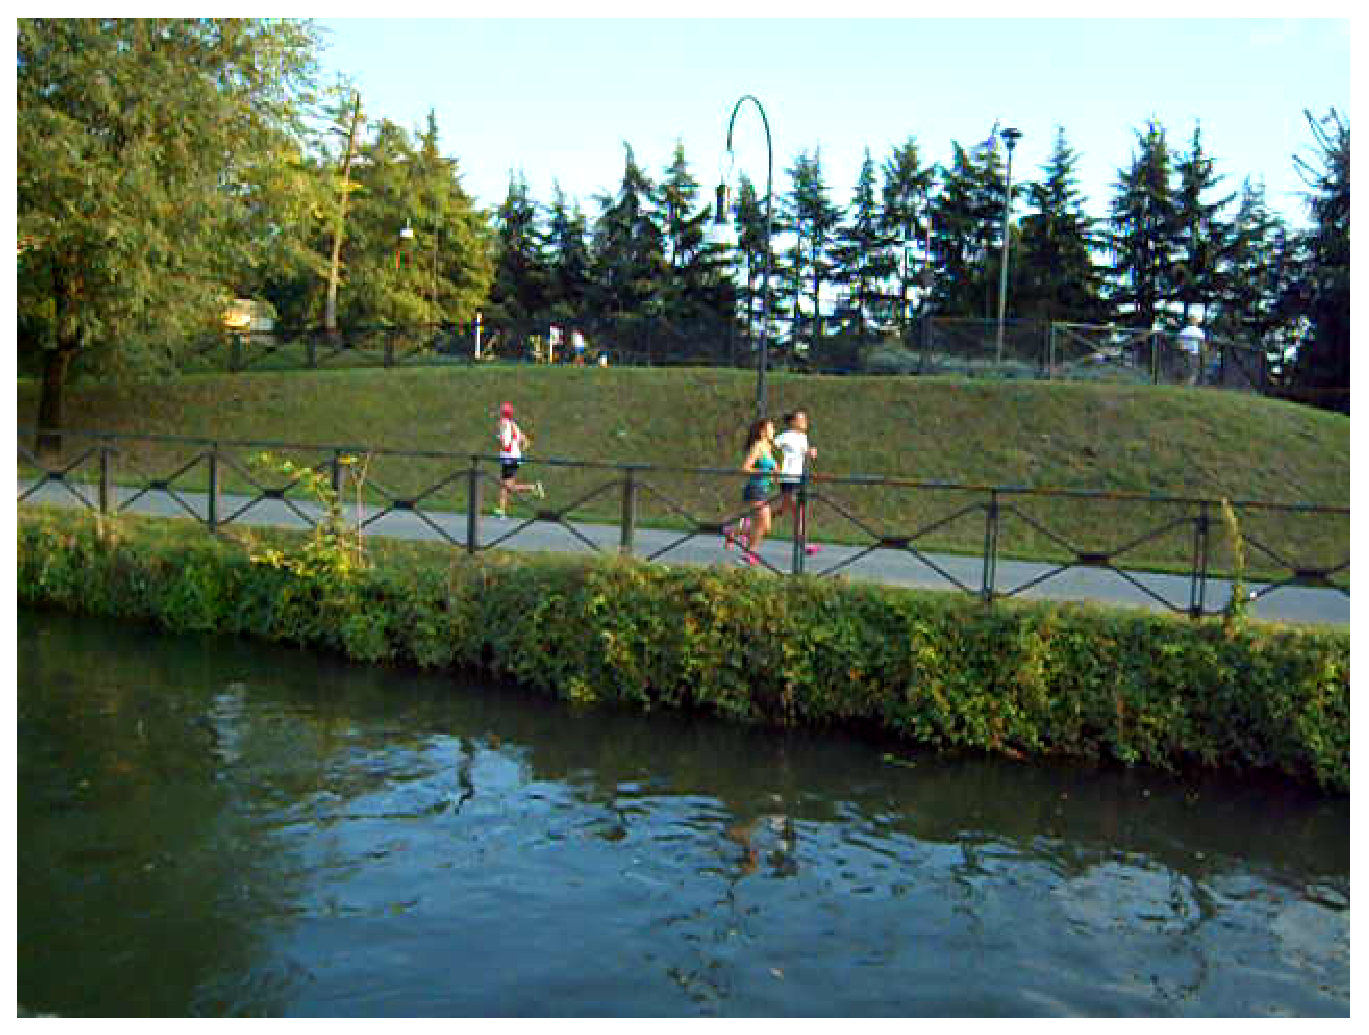
\includegraphics[width=6cm]{./pictures/FeatureVector/frame}}
	\end{subfigure}
	\begin{subfigure}[]
		{\label{fig:CLUSTERbrutto} 
\includegraphics[width=6cm]{./pictures/segmentazione/kmeansNormale}}
	\end{subfigure}
	\begin{subfigure}[]
		{\label{fig:risultatoClustering} 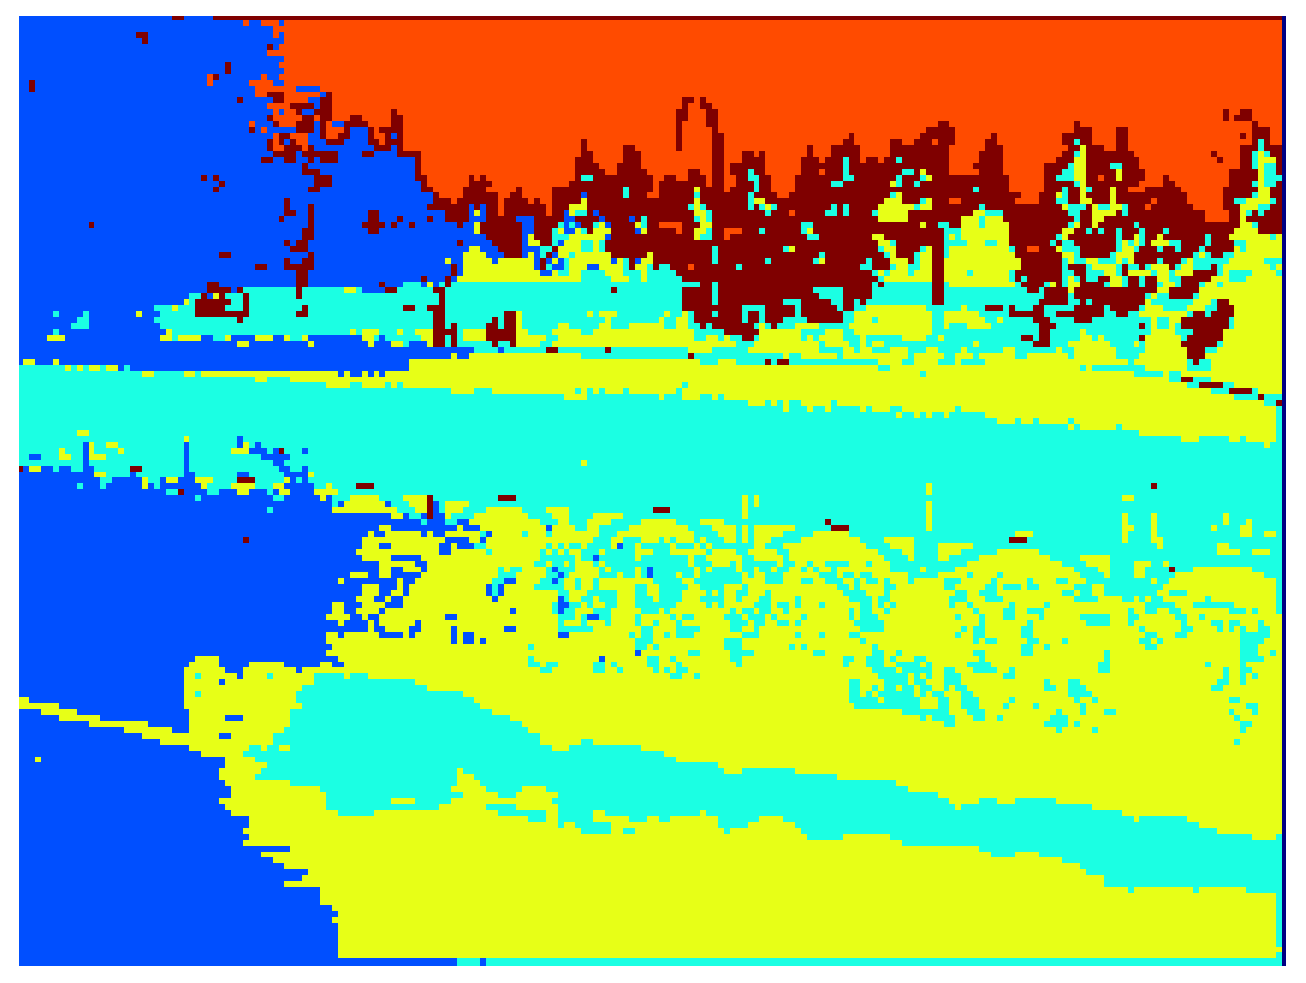
\includegraphics[width=6cm]{./pictures/segmentazione/mappa1}}
	\end{subfigure}
	\begin{subfigure}[]
		{\label{fig:mappaFinale} 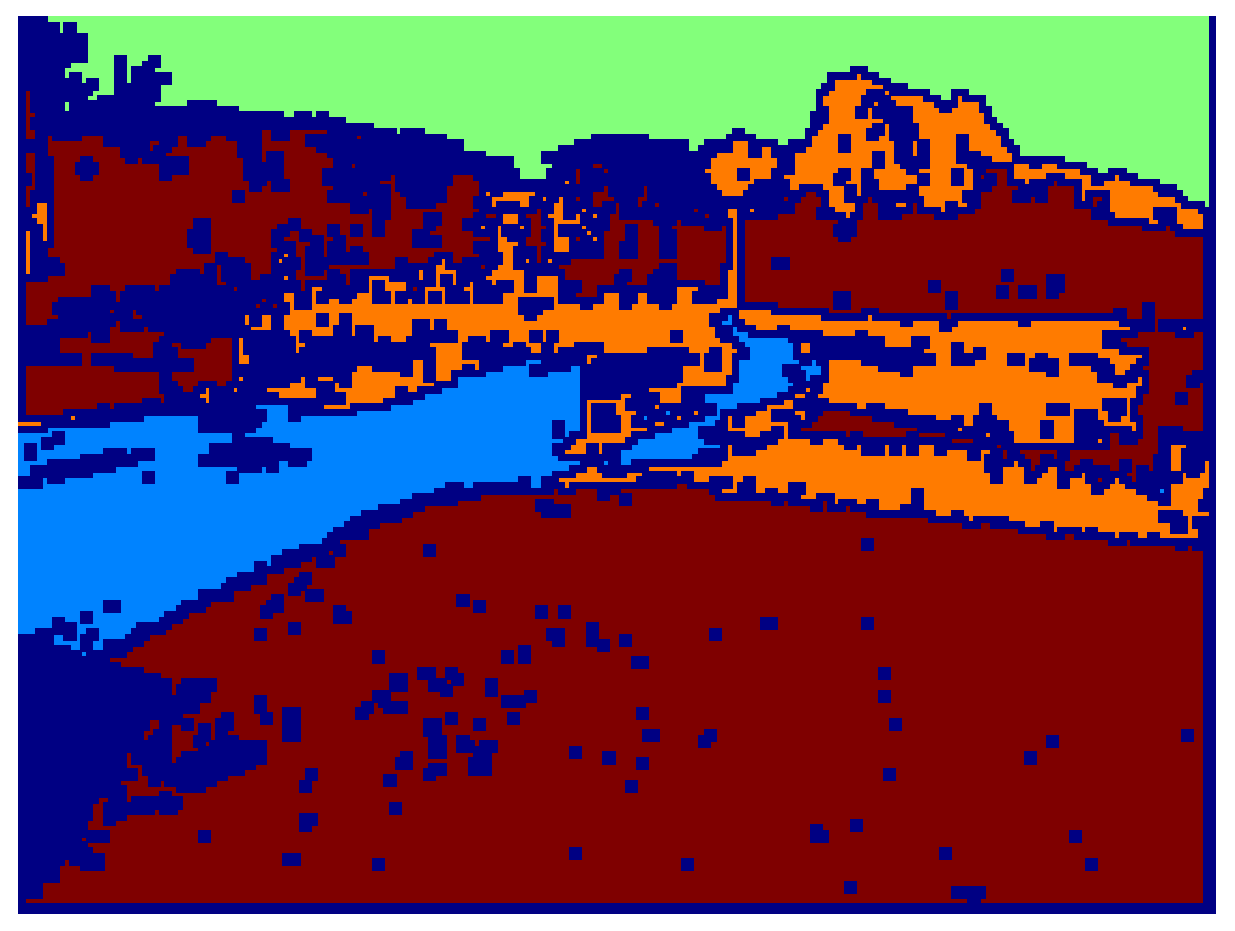
\includegraphics[width=6cm]{./pictures/segmentazione/mappa2}}
	\end{subfigure}
	\caption[Segmentazione della scena]{Un esempio di segmentazione di una particolare scena. 
		La scena di esempio \`e rappresentata in (a).
		Possiamo vedere in (b) il risultato della segmentazione utilizzando l'algoritmo di k-means nella sua versione originale, dove l'unico contributo \`e dato dalle coordinate dei pixel.
		Il risultato ottenuto utilizzando l'algoritmo di k-means pesato \`e illustrato invece in (c), dove possiamo vedere come la segmentazione sia legata a particolari regioni della scena.
		Infine, in (d) possiamo vedere il risultato finale della segmentazione, che consiste nella separazione della regioni e nell'eliminazione delle aree pi\`u piccole.}
	\label{fig:clustering}
\end{figure}
Per risolvere il problema abbiamo utilizzato, quindi una variante \textit{pesata} del k-means \cite{kottke1994motion}, in cui il calcolo delle distanze di ciascun dato da ogni centroide viene modificato associando un \textit{peso} a ciascuna componente:
\[{\dist}_{\text{w}}(\textbf{d}(\textbf{x}), \textbf{c}_i)=(\textbf{d}(\textbf{x}) - \textbf{c}_i)^TW^i(\textbf{d}(\textbf{x})-\textbf{c}_i),\]
dove $W^i$ \`e una matrice di pesi associata a ciascun cluster $C_i$:
\[W^i =
\left[\begin{array}{ccccc}
w_1^i & 0 & 0 & 0 & 0\\
0 & w_2^i & 0 & 0 & 0\\
0 & 0 & w_3^i& 0 & 0\\
0 & 0 & 0 & w_4^i & 0\\
0  & 0 & 0 & 0& w_5^i\\
\end{array}\right],
\]
dove $w_s^i$ corrisponde al peso dato all'elemento $s$ del feature vector associato al cluster $C_i$:
\[w_s^i= \frac{\left(\sigma_1^i \cdot \sigma_2^i \cdot \sigma_3^i\cdot \sigma_4^i\cdot \sigma_5^i\right)^{1/5}}{\sigma_s^i}, s=1,\dots,5,\] 
dove $\sigma_s^i$ rappresenta la deviazione standard dell'elemento $s$ dei dati appartenenti al cluster $C_i$.
\subsection{Separazione e rifinitura delle regioni}
L'algoritmo di clustering utilizzato produce un partizionamento della scena ripresa dalla camera come quello in Figura \ref{fig:risultatoClustering}.
Come possiamo vedere le regioni estratte dal nostro algoritmo sono legate a particolari aree presenti nella scena, in base alla loro dinamicit\`a, alla presenza di dettagli e all'intensit\`a media della luma.\\
La fase finale della segmentazione consiste nell'eliminare le regioni pi\`u piccole e separare quelle rimanenti per mezzo di \textit{operatori morfologici}.\\
La prima operazione che facciamo consiste nel separare le varie regioni tra di loro utilizzando l'operatore morfologico di \textit{erosione}.
Dato che l'operatore funziona su immagini \textit{binarie} creiamo, per ciascun cluster, una \textit{maschera binaria}:
\[M_i(x) =  \left\{ \begin{array}{rcl}
1 & \mbox{se} & x \in C_i \\
0 & \mbox{se} & x \notin C_i
\end{array}\right. , \forall x \in \mathcal{X}.\]
L'operatore morfologico di erosione esegue un filtraggio non lineare che rimpiazza il valore di ciascun pixel della maschera $M_i$ con il valore minimo tra quelli presenti in un suo intorno.
\[E_i(x) =  \left\{ \begin{array}{rcl}
1 & \mbox{se} & \forall \xi \in U_x \quad M_i(\xi) = 1 \\
0 & \mbox{se} & \exists \xi \in U_x \quad M_i(\xi) = 0
\end{array}\right. , \forall x \in \mathcal{X},\]
dove abbiamo indicato con $U_x$ l'intorno del pixel $x$.
Il risultato di questo operatore \`e quello di ridurre i bordi degli elementi posti a $1$ delle immagini binarie.\\
L'immagine binaria $E_i$ conterr\`a al suo interno un certo numero di \textit{regioni connesse}.
Le regioni pi\`u piccole, ovvero quelle il cui numero di pixel \`e inferiore allo $0,01\%$ dei pixel totali, vengono eliminate ponendo a $0$ il valore dei loro pixel.
Una volta eseguite queste operazioni su tutte le maschere $M_i$, i risultati finali vengono composti assieme in una nuova immagine:
\[ S(x)= \left\{ \begin{array}{rcll}
i & \mbox{se }  x \in E_i, & i=1,\dots,K \\
0 & \mbox{altrimenti} 
\end{array}\right. , \forall x \in \mathcal{X}.\]
Infine eliminiamo i cluster pi\`u piccoli, ovvero quelli il cui numero di pixel \`e inferiore al $2\%$ dei pixel totali.   
Il risultato finale \`e quello mostrato in Figura \ref{fig:mappaFinale}, dove le zone colorate in blu scuro rappresentano le aree che non vengono appartengono ad alcun cluster.
Queste zone, durante l'esecuzione dell'algoritmo di identificazione di spostamenti della camera, non verranno considerate nel calcolo dell'energia media della luma.
